%%%%%%%%%%%%%%%%%%%%%%%%%%%
%%  Componenti del back end
%%%%%%%%%%%%%%%%%%%%%%%%%%%



\subsection{\nogloxy{swedesigner::server}}
\label{\nogloxy{swedesigner::server}}
\subsubsection{Informazioni generali}
\begin{itemize}
\item \textbf{Descrizione}\\
Questo package contiene le componenti del server, scritte in Java.
\item \textbf{Padre}: \hyperref[\nogloxy{swedesigner}]{\nogloxy{\texttt{swedesigner}}}
\item \textbf{Package contenuti}:
\begin{itemize}
\item \hyperref[\nogloxy{swedesigner::server::compiler}]{\nogloxy{\texttt{compiler}}}\\
Questo package contiene le classi adibite alla compilazione del codice sorgente in codice eseguibile (nel linguaggio target specifico). È stata prevista la possibilità di ampliare questo package inserendo al suo interno ulteriori package. All'interno di questo package è presente unicamente il package \texttt{java}.
\item \hyperref[\nogloxy{swedesigner::server::controller}]{\nogloxy{\texttt{controller}}}\\
Questo package contiene i vari controller che implementano il pattern Front Controller fornito dal framework \emph{Spring}. Ogni controller dovrebbe occuparsi di gestire una richiesta e di rispondere opportunamente ad essa, attraverso l'interfaccia REST definita.
\item \hyperref[\nogloxy{swedesigner::server::generator}]{\nogloxy{\texttt{generator}}}\\
Questo package contiene le classi adibite alla trasformazione dal diagramma (rappresentato in oggetti Java derivati da oggetti JSON) a codice sorgente, nel linguaggio target specifico. È stata prevista la possibilità di ampliare questo package inserendo al suo interno ulteriori package. All'interno di questo package è presente unicamente il package \texttt{java}.
\item \hyperref[\nogloxy{swedesigner::server::parser}]{\nogloxy{\texttt{parser}}}\\
Questo package presenta le classi utili all'attività di parsing dei dati ricevuti dai client.
\item \hyperref[\nogloxy{swedesigner::server::project}]{\nogloxy{\texttt{project}}}\\
Questo package contiene al suo interno le classi utili a rappresentare un progetto UML. Il package parser necessita di questo package per poter dare in output un programma rappresentato in memoria come oggetti Java. Per chiarezza e per evitare l'uso di keyword riservate dal linguaggio Java, all'inizio del nome di queste classi è inserito il prefisso \texttt{Parsed} (e.g. \texttt{ParsedClass}).
\item \hyperref[\nogloxy{swedesigner::server::stereotype}]{\nogloxy{\texttt{stereotype}}}\\
Questo package offre le classi che descrivono ciò che caratterizza un particolare stereotipo. Queste classi derivano tutte da una classe base chiamata \texttt{Stereotype}. Le classi che definiscono come deve variare ogni stereotipo sono contraddistinte dal suffisso \texttt{Stereotype} (e.g. \texttt{BoardStereotype}). Si noti che tra queste classi non sono presenti dei legami, in quanto sono necessarie alla generazione del codice. La struttura degli stereotipi assegnabili ad ogni classe e le loro relazioni saranno definite successivamente nella \emph{Definizione di Prodotto}.
\item \hyperref[\nogloxy{swedesigner::server::template}]{\nogloxy{\texttt{template}}}\\
Questo package contiene le classi necessarie a trasformare l'oggetto che rappresenta il programma in una stringa di testo che rappresenta il codice sorgente tramite un sistema a template, il quale definirà tramite dei file di testo la struttura di ogni componente del programma; per facilitare questo compito sarà usata la libreria \stringtemplate{}. Similarmente al package \texttt{Generator} si è prevista la possibilità di implementare un sistema di template per ogni linguaggio, implementando diversamente l'interfaccia della classe Template e definendo un nuovo package (e.g. \texttt{Java}).
\item \hyperref[\nogloxy{swedesigner::server::utility}]{\nogloxy{\texttt{utility}}}\\
Questo package contiene le componenti secondarie necessarie al server, indipendentemente dal linguaggio target dell'applicazione.
\end{itemize}
\end{itemize}
\subsubsection{Classi}
\subsubsubsection{\nogloxy{swedesigner::server::Application}}
\label{\nogloxy{swedesigner::server::Application}}
\begin{figure}[h]
\centering
\nogloxy{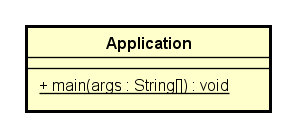
\includegraphics[scale=0.8,keepaspectratio]{img/server/Application.png}}
\caption{\nogloxy{swedesigner::server::Application}}
\end{figure}
\FloatBarrier
\begin{itemize}
\item \textbf{Descrizione}\\
Classe principale che consente l'avvio dell'applicazione spring.
\item \textbf{Utilizzo}\\
La classe viene utilizzata per avviare l'applicazione spring
\item \textbf{Metodi}:
\begin{itemize}
\item \nogloxy{\texttt{+ main(args: String[]): void}}
\\ Metodo principale che permette l'avvio dell'applicazione spring
\\ \textbf{Parametri}:
\begin{itemize}
\item \nogloxy{\texttt{args: String[]}}
\\ Rappresenta gli eventuali parametri passa al programma.
\end{itemize}
\end{itemize}
\end{itemize}
\subsection{\nogloxy{swedesigner::server::compiler}}
\label{\nogloxy{swedesigner::server::compiler}}
\subsubsection{Informazioni generali}
\begin{itemize}
\item \textbf{Descrizione}\\
Questo package contiene le classi adibite alla compilazione del codice sorgente in codice eseguibile (nel linguaggio target specifico). È stata prevista la possibilità di ampliare questo package inserendo al suo interno ulteriori package. All'interno di questo package è presente unicamente il package \texttt{java}.
\item \textbf{Padre}: \hyperref[\nogloxy{swedesigner::server}]{\nogloxy{\texttt{server}}}
\item \textbf{Package contenuti}:
\begin{itemize}
\item \hyperref[\nogloxy{swedesigner::server::compiler::java}]{\nogloxy{\texttt{java}}}\\
Questo package offre un'implementazione dell'interfaccia \texttt{Compiler} appartenente al package superiore. Possono essere aggiunti simili package per permettere la generazione in altri linguaggi.
\end{itemize}
\end{itemize}
\subsubsection{Classi}
\subsubsubsection{\nogloxy{swedesigner::server::compiler::Compiler}}
\label{\nogloxy{swedesigner::server::compiler::Compiler}}
\begin{figure}[h]
\centering
\nogloxy{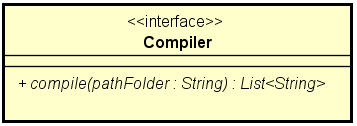
\includegraphics[scale=0.8,keepaspectratio]{img/server/Compiler.png}}
\caption{\nogloxy{swedesigner::server::compiler::Compiler}}
\end{figure}
\FloatBarrier
\begin{itemize}
\item \textbf{Descrizione}\\
questa interfaccia si occupa di fornire un oggetto compiler generico a chi lo richiede in modo da poter rendere entensibile il sistema aggiungendo un'implementazione concreta del compiler del linguaggio target desiderato.
\item \textbf{Utilizzo}\\
\textt{RequestHandlerController} ha una dipendenza verso \texttt{Compiler} in quanto chiederà a \textt{CompilerAssembler} una implementazione concreta di un \textt{Compiler} in base al linguaggio target. Il pattern realizzato con questa classe è una \emph{dependency injection}.
\item \textbf{Relazioni con altre classi}:
\begin{itemize}
\item \textit{IN} \hyperref[\nogloxy{swedesigner::server::compiler::java::JavaCompiler}]{\nogloxy{\texttt{JavaCompiler}}}\\
questa classe è una implementazione di \texttt{Compiler} che permette di creare un jar dal codice sorgente Java.
\item \textit{IN} \hyperref[\nogloxy{swedesigner::server::controller::RequestHandlerController}]{\nogloxy{\texttt{RequestHandlerController}}}\\
questa classe si occupa di ricevere le richieste REST provenienti dal client.
\end{itemize}
\item \textbf{Metodi}:
\begin{itemize}
\item \nogloxy{\texttt{+ compile(pathFolder: String): List<String>}}
\\ Compila un file sorgente in un eseguibile; ritorna una lista di errori di compilazione, se ce ne sono.
\\ \textbf{Parametri}:
\begin{itemize}
\item \nogloxy{\texttt{pathFolder: String}}
\\ Rappresenta la posizione della cartella nella quale sono presenti i file sorgente da compilare, relativi ad una particolare richiesta.
\end{itemize}
\end{itemize}
\end{itemize}
\subsection{\nogloxy{swedesigner::server::compiler::java}}
\label{\nogloxy{swedesigner::server::compiler::java}}
\subsubsection{Informazioni generali}
\begin{itemize}
\item \textbf{Descrizione}\\
Questo package offre un'implementazione dell'interfaccia \texttt{Compiler} appartenente al package superiore. Possono essere aggiunti simili package per permettere la generazione in altri linguaggi.
\item \textbf{Padre}: \hyperref[\nogloxy{swedesigner::server::compiler}]{\nogloxy{\texttt{compiler}}}
\end{itemize}
\subsubsection{Classi}
\subsubsubsection{\nogloxy{swedesigner::server::compiler::java::JavaCompiler}}
\label{\nogloxy{swedesigner::server::compiler::java::JavaCompiler}}
\begin{figure}[h]
\centering
\nogloxy{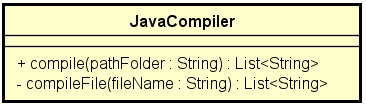
\includegraphics[scale=0.8,keepaspectratio]{img/server/JavaCompiler.png}}
\caption{\nogloxy{swedesigner::server::compiler::java::JavaCompiler}}
\end{figure}
\FloatBarrier
\begin{itemize}
\item \textbf{Descrizione}\\
questa classe è una implementazione di \texttt{Compiler} che permette di creare un jar dal codice sorgente Java.
\item \textbf{Utilizzo}\\
viene utilizzata da \texttt{CompilerAssembler} che ritorna un' istanza di essa quando richiesto.
\item \textbf{Relazioni con altre classi}:
\begin{itemize}
\item \textit{OUT} \hyperref[\nogloxy{swedesigner::server::compiler::Compiler}]{\nogloxy{\texttt{Compiler}}}\\
questa interfaccia si occupa di fornire un oggetto compiler generico a chi lo richiede in modo da poter rendere entensibile il sistema aggiungendo un'implementazione concreta del compiler del linguaggio target desiderato.
\end{itemize}
\item \textbf{Metodi}:
\begin{itemize}
\item \nogloxy{\texttt{+ compile(pathFolder: String): List<String>}}
\\ Crea i file compilati con estensione .class relativi ai file sorgente .java contenuti nella cartella che ha come percorso la stringa passata alla funzione stessa.
\\ \textbf{Parametri}:
\begin{itemize}
\item \nogloxy{\texttt{pathFolder: String}}
\\ Rappresenta la posizione della cartella nella quale sono presenti i file sorgente .java da compilare, relativi ad una particolare richiesta.
\end{itemize}
\item \nogloxy{\texttt{- compileFile(fileName: String): List<String>}}
\\ Crea il file compilato con estensione .class relativo al file sorgente .java passato come parametro.
\\ \textbf{Parametri}:
\begin{itemize}
\item \nogloxy{\texttt{fileName: String}}
\\ Rappresenta il percorso di un file con estensione .java.
\end{itemize}
\end{itemize}
\end{itemize}
\subsection{\nogloxy{swedesigner::server::controller}}
\label{\nogloxy{swedesigner::server::controller}}
\subsubsection{Informazioni generali}
\begin{itemize}
\item \textbf{Descrizione}\\
Questo package contiene i vari controller che implementano il pattern Front Controller fornito dal framework \emph{Spring}. Ogni controller dovrebbe occuparsi di gestire una richiesta e di rispondere opportunamente ad essa, attraverso l'interfaccia REST definita.
\item \textbf{Padre}: \hyperref[\nogloxy{swedesigner::server}]{\nogloxy{\texttt{server}}}
\end{itemize}
\subsubsection{Classi}
\subsubsubsection{\nogloxy{swedesigner::server::controller::RequestHandlerController}}
\label{\nogloxy{swedesigner::server::controller::RequestHandlerController}}
\begin{figure}[h]
\centering
\nogloxy{\includegraphics[scale=0.4,keepaspectratio]{img/server/handleGenerationRequestSequence.png}}
\caption{\nogloxy{diagramma di sequenza per le interazioni fra classi gestite dal metodo handleGenerationRequest}}
\end{figure}

\begin{figure}[h]
\centering
\nogloxy{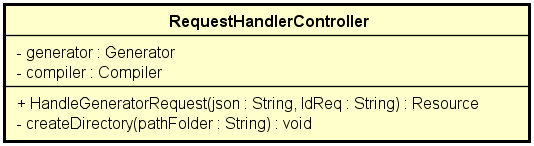
\includegraphics[scale=0.8,keepaspectratio]{img/server/RequestHandlerController.png}}
\caption{\nogloxy{swedesigner::server::controller::RequestHandlerController}}
\end{figure}
\FloatBarrier
\begin{itemize}
\item \textbf{Descrizione}\\
questa classe si occupa di ricevere le richieste REST provenienti dal client.
\item \textbf{Utilizzo}\\
essa deve gestire la richiesta di generazione di un progetto (attraverso file JSON) generando il codice e ritornandolo all'utente; inoltre essa deve restituire l'elenco degli stereotipi esistenti all'interno del server, con meta-attributi e meta-classi.
Richiama in ordine le varie classi addette alla generazione del codice, ovvero: un \texttt{Parser}, un \texttt{Generator}, un \texttt{Compiler} e infine il \texttt{Compressor}. 
\item \textbf{Relazioni con altre classi}:
\begin{itemize}
\item \textit{OUT} \hyperref[\nogloxy{swedesigner::server::compiler::Compiler}]{\nogloxy{\texttt{Compiler}}}\\
questa interfaccia si occupa di fornire un oggetto compiler generico a chi lo richiede in modo da poter rendere entensibile il sistema aggiungendo un'implementazione concreta del compiler del linguaggio target desiderato.
\item \textit{OUT} \hyperref[\nogloxy{swedesigner::server::generator::Generator}]{\nogloxy{\texttt{Generator}}}\\
questa interfaccia si occupa di fornire un oggetto \texttt{Generator} generico a chi lo richiede in modo da poter rendere entensibile il sistema aggiungendo un'implementazione concreta del generator del linguaggio target desiderato.
\item \textit{OUT} \hyperref[\nogloxy{swedesigner::server::parser::Parser}]{\nogloxy{\texttt{Parser}}}\\
questa classe si occupa di elaborare il file JSON proveniente dal client e di creare da esso un oggetto Java \texttt{ParsedProgram} strutturato in modo da poter essere facilmente convertito in codice.
\item \textit{OUT} \hyperref[\nogloxy{swedesigner::server::utility::Compressor}]{\nogloxy{\texttt{Compressor}}}\\
questa classe si occupa di creare e salvare su disco un archivio compresso contenente il progetto JSON, il codice sorgente e l'eseguibile generato che verrà poi messo a disposizione dell'utente che potrà scaricarlo.
\end{itemize}
\item \textbf{Attributi}:
\begin{itemize}
\item \nogloxy{\texttt{- compiler: Compiler}}
\\ Rifermento all'istanza di Compiler da utilizzare
\item \nogloxy{\texttt{- compressor: Compressor}}
\\ Riferimento all'istanza di Compressor da utilizzare.
\item \nogloxy{\texttt{- parser: Parser}}
\\ Riferimento all'istanza di Parser da utilizzare.
\item \nogloxy{\texttt{- uploadFolder: String}}
\\ Percorso della cartella all'interno del server nella quale memorizzare l'archivio zip da ritornare all'utente.
\item \nogloxy{\texttt{- generator: Generator}}
\\ Riferimento all'istanza di Generator da utilizzare.
\end{itemize}
\item \textbf{Metodi}:
\begin{itemize}
\item \nogloxy{\texttt{- createDirectory(pathFolder: String): void}}
\\ Gestisce la creazione di un'apposita cartella per la particolare richiesta ricevuta.
\\ \textbf{Parametri}:
\begin{itemize}
\item \nogloxy{\texttt{pathFolder: String}}
\\ Rappresenta la posizione della cartella che verrà creata relativa ad una particolare richiesta.
\end{itemize}
\item \nogloxy{\texttt{+ handleGenerationRequest(httpEntity: HttpEntity<String>): ResponseEntity<?>}}

\item \nogloxy{\texttt{+ HandleGenerationRequest(json: String, IdReq: String): void}}
\\ Il metodo riceve a partire dalla richiesta del client una stringa in formato .json ed anche l'id della richiesta stessa.
Il suo compito è:
\begin{itemize}
\item istanziare un oggetto Parser ed invocare su di esso il metodo createParsedProgram passando come argomento il file .json;
\item invocare il metodo generate sul proprio riferimento di tipo Generator passando come riferimento il ParsedProgram così ottenuto;
\item invocare sull'attributo compiler il metodo compile passando come argomento il riferimento alla cartella relativa alla particolare richiesta all'interno del server contenente i file .java;
\item istanziare un oggetto Compressor ed invocare su di esso il metodo zip per realizzare la risorsa .zip da ritornare all'utente;
\item ritornare in risposta all'utente il link a partire dal quale scaricare la risorsa .zip desiderata oppure un messaggio contenente gli errori rilevati dal Parser o dal Generator.
\end{itemize}
 \textbf{Parametri}:
\begin{itemize}
\item \nogloxy{\texttt{httpEntity: HttpEntity<String>}}
\\ Richiesta http contenente il file .json prodotto dall'editor.
\end{itemize}
\end{itemize}
\end{itemize}
\subsection{\nogloxy{swedesigner::server::generator}}
\label{\nogloxy{swedesigner::server::generator}}
\subsubsection{Informazioni generali}
\begin{itemize}
\item \textbf{Descrizione}\\
Questo package contiene le classi adibite alla trasformazione dal diagramma (rappresentato in oggetti Java derivati da oggetti JSON) a codice sorgente, nel linguaggio target specifico. È stata prevista la possibilità di ampliare questo package inserendo al suo interno ulteriori package. All'interno di questo package è presente unicamente il package \texttt{java}.
\item \textbf{Padre}: \hyperref[\nogloxy{swedesigner::server}]{\nogloxy{\texttt{server}}}
\item \textbf{Package contenuti}:
\begin{itemize}
\item \hyperref[\nogloxy{swedesigner::server::generator::java}]{\nogloxy{\texttt{java}}}\\
Questo package offre un'implementazione dell'interfaccia \texttt{Generator} appartenente al package superiore. Possono essere aggiunti simili package per permettere la generazione in altri linguaggi.
\end{itemize}
\end{itemize}
\subsubsection{Classi}
\subsubsubsection{\nogloxy{swedesigner::server::generator::Generator}}
\label{\nogloxy{swedesigner::server::generator::Generator}}
\begin{figure}[h]
\centering
\nogloxy{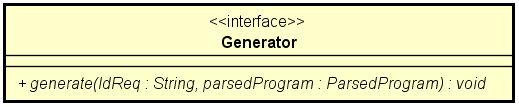
\includegraphics[scale=0.8,keepaspectratio]{img/server/Generator.png}}
\caption{\nogloxy{swedesigner::server::generator::Generator}}
\end{figure}
\FloatBarrier
\begin{itemize}
\item \textbf{Descrizione}\\
questa interfaccia si occupa di fornire un oggetto \texttt{Generator} generico a chi lo richiede in modo da poter rendere entensibile il sistema aggiungendo un'implementazione concreta del generator del linguaggio target desiderato.
\item \textbf{Utilizzo}\\
\texttt{RequestHandlerController} ha una dipendenza verso \texttt{Generator} in quanto chiederà a \texttt{GeneratorAssembler} una implementazione concreta di un \texttt{Generator} in base al linguaggio target. Il pattern realizzato con questa classe è una \emph{dependency injection}.
\item \textbf{Relazioni con altre classi}:
\begin{itemize}
\item \textit{IN} \hyperref[\nogloxy{swedesigner::server::controller::RequestHandlerController}]{\nogloxy{\texttt{RequestHandlerController}}}\\
questa classe si occupa di ricevere le richieste REST provenienti dal client.
\item \textit{IN} \hyperref[\nogloxy{swedesigner::server::generator::java::JavaGenerator}]{\nogloxy{\texttt{JavaGenerator}}}\\
questa classe è una implementazione di \texttt{Compiler} che permette di creare del codice sorgente Java da un \texttt{ParsedProgram}.
\item \textit{OUT} \hyperref[\nogloxy{swedesigner::server::project::ParsedElement}]{\nogloxy{\texttt{ParsedElement}}}\\
questa classe descrive il contratto di un elemento generico \texttt{Parsed}. Si specifica il metodo \texttt{RenderTemplate} che impone la necessità di implementarlo ad ogni classe sottostante.
\item \textit{OUT} \hyperref[\nogloxy{swedesigner::server::template::Template}]{\nogloxy{\texttt{Template}}}\\
questa interfaccia si occupa di fornire un oggetto template generico a chi lo richiede in modo da poter rendere estensibile il sistema aggiungendo un'implementazione concreta del template del linguaggio target desiderato.
\end{itemize}
\item \textbf{Metodi}:
\begin{itemize}
\item \nogloxy{\texttt{+ generate(idReq: String, parsedProgram: ParsedProgram): void}}
\\ Crea e salva i file sorgente del programma.
\\ \textbf{Parametri}:
\begin{itemize}
\item \nogloxy{\texttt{idReq: String}}
\\ Rappresenta l'identificatore della richiesta ricevuta.
\item \nogloxy{\texttt{parsedProgram: ParsedProgram}}
\\ Rappresenta l'oggetto ParsedProgram che sarà trasformato nel codice di un particolare linguaggio. 
\end{itemize}
\end{itemize}
\end{itemize}
\subsection{\nogloxy{swedesigner::server::generator::java}}
\label{\nogloxy{swedesigner::server::generator::java}}
\subsubsection{Informazioni generali}
\begin{itemize}
\item \textbf{Descrizione}\\
Questo package offre un'implementazione dell'interfaccia \texttt{Generator} appartenente al package superiore. Possono essere aggiunti simili package per permettere la generazione in altri linguaggi.
\item \textbf{Padre}: \hyperref[\nogloxy{swedesigner::server::generator}]{\nogloxy{\texttt{generator}}}
\end{itemize}
\subsubsection{Classi}
\subsubsubsection{\nogloxy{swedesigner::server::generator::java::JavaGenerator}}
\label{\nogloxy{swedesigner::server::generator::java::JavaGenerator}}
\begin{figure}[h]
\centering
\nogloxy{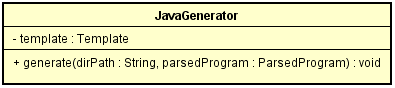
\includegraphics[scale=0.8,keepaspectratio]{img/server/JavaGenerator.png}}
\caption{\nogloxy{swedesigner::server::generator::java::JavaGenerator}}
\end{figure}
\FloatBarrier
\begin{itemize}
\item \textbf{Descrizione}\\
questa classe è una implementazione di \texttt{Compiler} che permette di creare del codice sorgente Java da un \texttt{ParsedProgram}.
\item \textbf{Utilizzo}\\
viene utilizzata da \texttt{CompilerAssembler} che ritorna un' istanza di essa quando richiesto.
\item \textbf{Relazioni con altre classi}:
\begin{itemize}
\item \textit{OUT} \hyperref[\nogloxy{swedesigner::server::generator::Generator}]{\nogloxy{\texttt{Generator}}}\\
questa interfaccia si occupa di fornire un oggetto \texttt{Generator} generico a chi lo richiede in modo da poter rendere entensibile il sistema aggiungendo un'implementazione concreta del generator del linguaggio target desiderato.
\end{itemize}
\item \textbf{Attributi}:
\begin{itemize}
\item \nogloxy{\texttt{- template: Template}}
\\ Riferimento alla particolare istanza di Template da utilizzare.
\end{itemize}
\item \textbf{Metodi}:
\begin{itemize}
\item \nogloxy{\texttt{+ generate(parsedProgram: ParsedProgram, idReq: String): void}}
\\ Crea e salva i file sorgente .java del programma.
\\ \textbf{Parametri}:
\begin{itemize}
\item \nogloxy{\texttt{parsedProgram: ParsedProgram}}
\\ Rappresenta l'oggetto ParsedProgram che sarà trasformato in codice Java. 
\item \nogloxy{\texttt{idReq: String}}
\\ Rappresenta l'identificatore della richiesta ricevuta.
\end{itemize}
\end{itemize}
\end{itemize}
\subsection{\nogloxy{swedesigner::server::parser}}
\label{\nogloxy{swedesigner::server::parser}}
\subsubsection{Informazioni generali}
\begin{itemize}
\item \textbf{Descrizione}\\
Questo package presenta le classi utili all'attività di parsing dei dati ricevuti dai client.
\item \textbf{Padre}: \hyperref[\nogloxy{swedesigner::server}]{\nogloxy{\texttt{server}}}
\end{itemize}
\subsubsection{Classi}
\subsubsubsection{\nogloxy{swedesigner::server::parser::Parser}}
\label{\nogloxy{swedesigner::server::parser::Parser}}
\begin{figure}[H]
\centering
\nogloxy{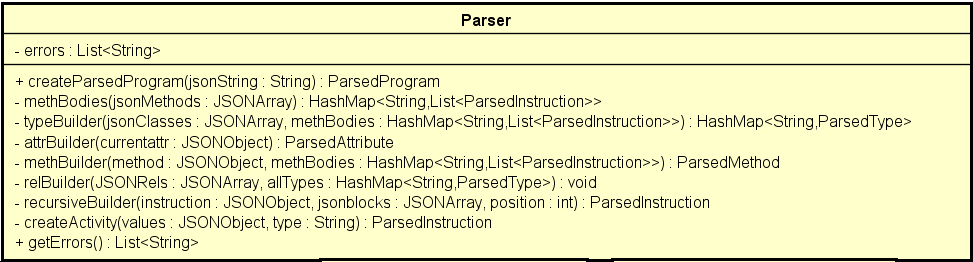
\includegraphics[scale=0.4,keepaspectratio]{img/server/Parser.png}}
\caption{\nogloxy{swedesigner::server::parser::Parser}}
\end{figure}
\begin{figure}[h]
\centering
\nogloxy{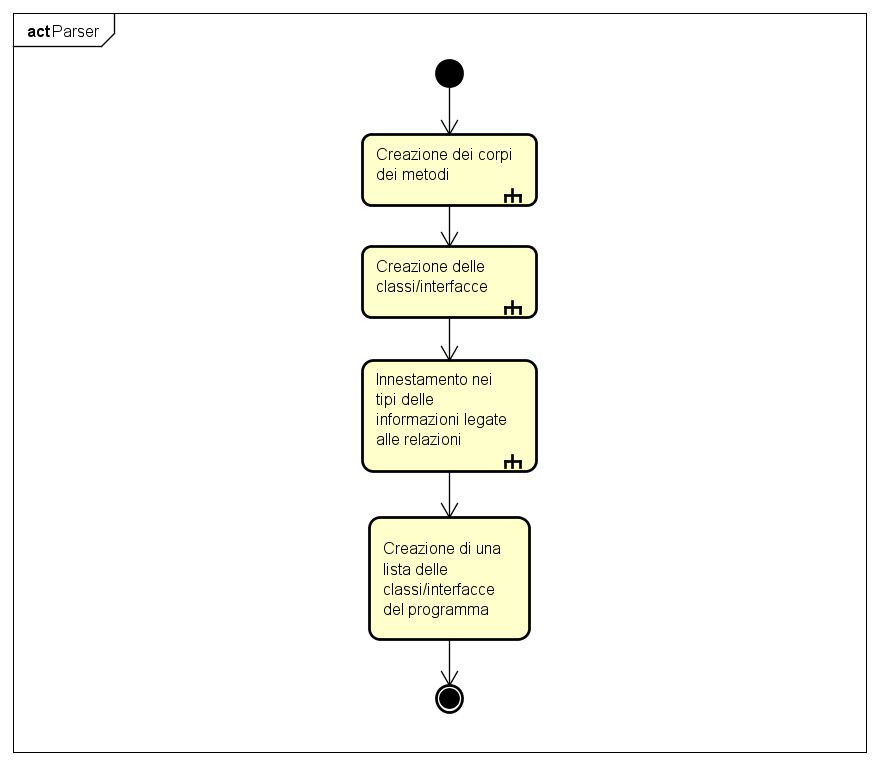
\includegraphics[scale=0.4,keepaspectratio]{img/server/ParserActivity.png}}
\caption{\nogloxy{diagramma di attività per il flusso di esecuzione del metodo createParsedProgram della classe Parser}}
\end{figure}
\begin{figure}[h]
\centering
\nogloxy{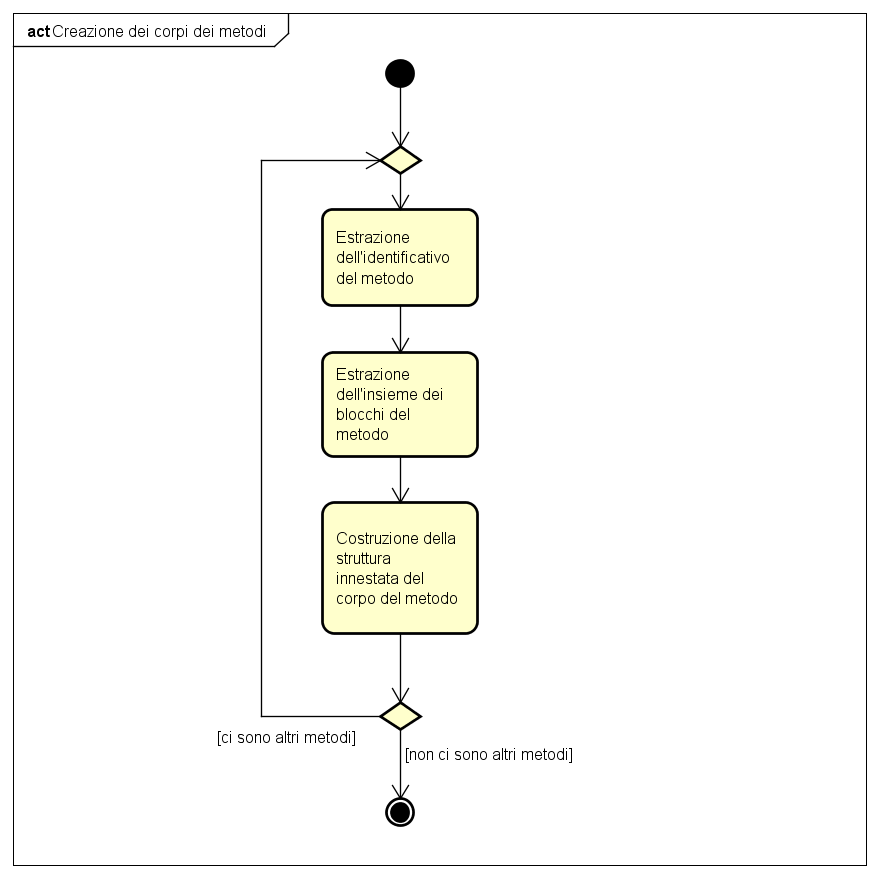
\includegraphics[scale=0.4,keepaspectratio]{img/server/CreazioneCorpiMetodiActivity.png}}
\caption{\nogloxy{diagramma di attività per il flusso di esecuzione del metodo methBuilder della classe Parser}}
\end{figure}
\begin{figure}[h]
\centering
\nogloxy{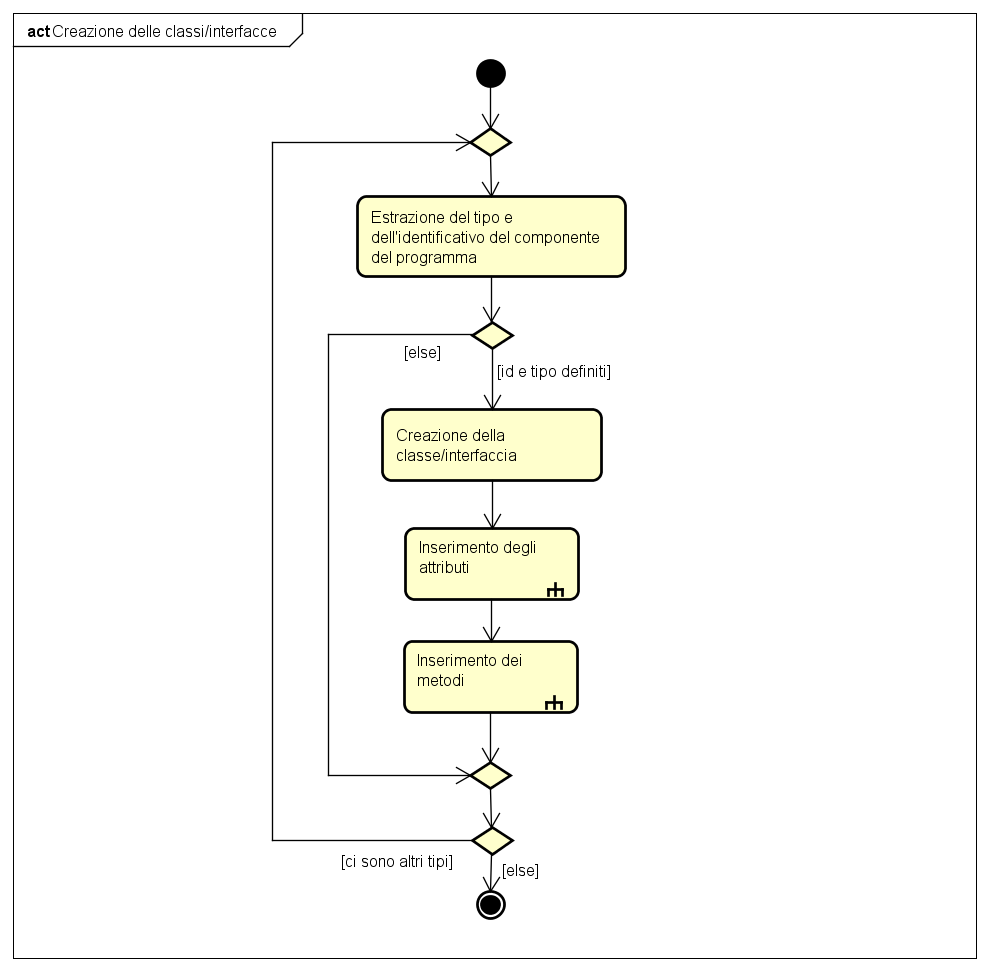
\includegraphics[scale=0.4,keepaspectratio]{img/server/CreazioneTipiActivity.png}}
\caption{\nogloxy{diagramma di attività per il flusso di esecuzione del metodo typeBuilder della classe Parser}}
\end{figure}
\begin{figure}[h]
\centering
\nogloxy{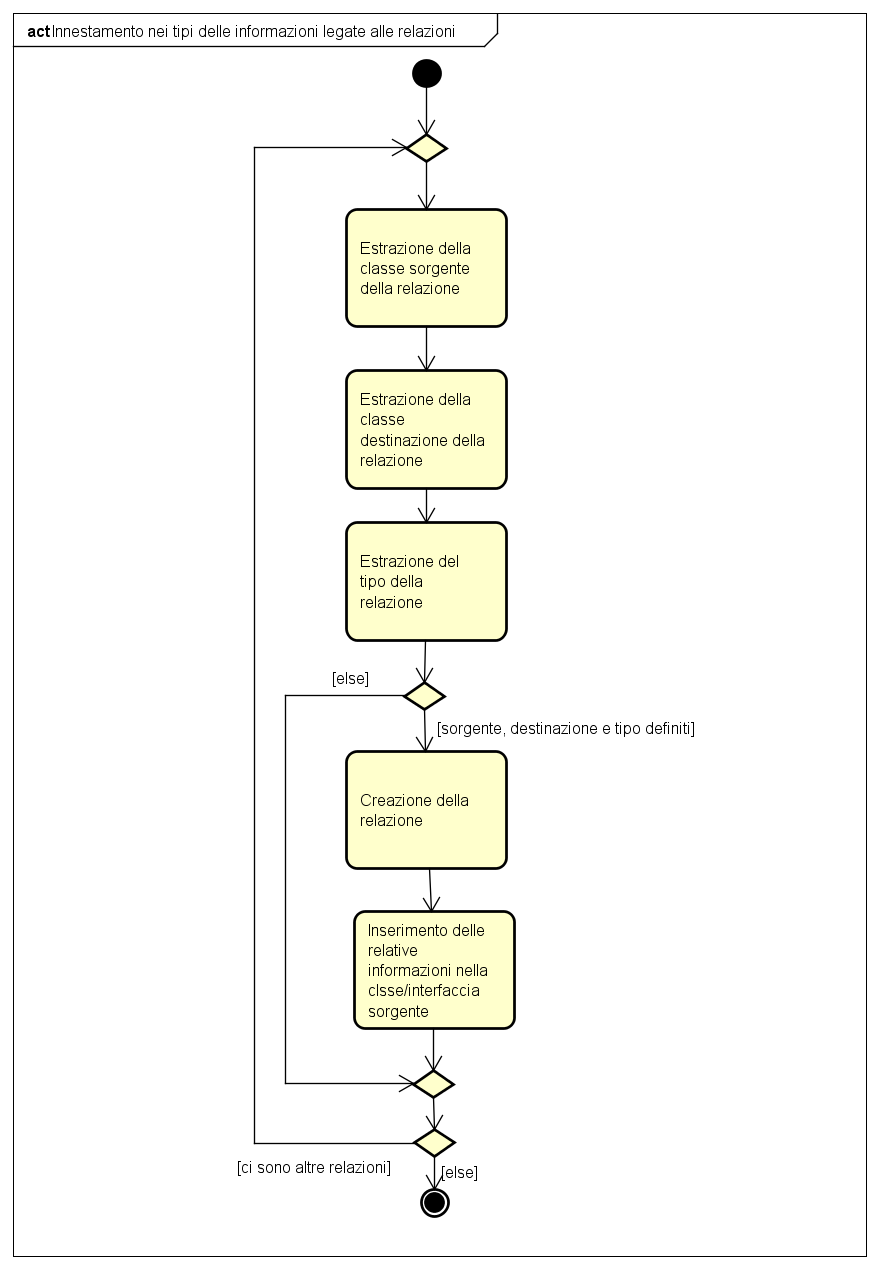
\includegraphics[scale=0.4,keepaspectratio]{img/server/CreazioneRelazioniActivity.png}}
\caption{\nogloxy{diagramma di attività per il flusso di esecuzione del metodo relBuilder della classe Parser}}
\end{figure}
\FloatBarrier
\begin{itemize}
\item \textbf{Descrizione}\\
questa classe si occupa di elaborare il file JSON proveniente dal client e di creare da esso un oggetto Java \texttt{ParsedProgram} strutturato in modo da poter essere facilmente convertito in codice.
\item \textbf{Utilizzo}\\
viene utilizzata da \texttt{RequestHandlerController} che ne crea un istanza e ne chiama i metodi per elaborare il JSON. \texttt{Parser} inoltre crea istanze di \texttt{ParsedElement} e ritorna a controller un'istanza di \texttt{ParsedProgram}.
\item \textbf{Relazioni con altre classi}:
\begin{itemize}
\item \textit{IN} \hyperref[\nogloxy{swedesigner::server::controller::RequestHandlerController}]{\nogloxy{\texttt{RequestHandlerController}}}\\
questa classe si occupa di ricevere le richieste REST provenienti dal client.
\item \textit{OUT} \hyperref[\nogloxy{swedesigner::server::project::ParsedProgram}]{\nogloxy{\texttt{ParsedProgram}}}\\
questa classe rappresenta l'entità che possiede al suo interno tutte le componenti di un progetto. Essa possiede più \texttt{ParsedType}.
\end{itemize}
\item \textbf{Attributi}:
\begin{itemize}
\item \nogloxy{\texttt{- errors: List<String>}}
\\ è la lista in cui vengono memorizzati gli errori rilevati durante l'elaborazione della stringa json.
\end{itemize}
\item \textbf{Metodi}:
\begin{itemize}
\item \nogloxy{\texttt{- attrBuilder(currentAttr: JSONObject): ParsedAttribute}}
\\ Costruisce l'oggetto relativo ad uno dei campi dati delle classi del programma.
\\ \textbf{Parametri}:
\begin{itemize}
\item \nogloxy{\texttt{currentAttr: JSONObject}}
\\ Rappresenta un attributo/campo dato in forma JSON.
\end{itemize}
\item \nogloxy{\texttt{- createActivity(value: JSONObject, type: String): ParsedInstruction}}
\\ Costruisce l'oggetto relativo ad una particolare istruzione del programma.
\\ \textbf{Parametri}:
\begin{itemize}
\item \nogloxy{\texttt{value: JSONObject}}
\\ Rappresenta un particolare blocco di istruzioni in forma JSON.
\item \nogloxy{\texttt{type: String}}
\\ Rappresenta il tipo di un particolare blocco di istruzioni.
\end{itemize}
\item \nogloxy{\texttt{+ createParsedProgram(jsonString: String): ParsedProgram}}
\\ Traduce la stringa json in una corrispondente struttura ad oggetti.
\\ \textbf{Parametri}:
\begin{itemize}
\item \nogloxy{\texttt{jsonString: String}}
\\ Rappresenta il contenuto del file .json in forma di stringa.
\end{itemize}
\item \nogloxy{\texttt{+ getErrors(): List<String>}}
\\ Ritorna l'attributo errors.
\item \nogloxy{\texttt{- methBodies(jsonMethods: JSONArray): HashMap<String, List<ParsedInstruction>}}
\\ Crea la struttura ad oggetti relativa al corpo dei metodi del programma.
\\ \textbf{Parametri}:
\begin{itemize}
\item \nogloxy{\texttt{jsonMethods: JSONArray}}
\\ Rappresenta l'insieme dei corpi dei metodi in forma JSON.
\end{itemize}
\item \nogloxy{\texttt{- methBuilder(method: JSONObject, methBodies: HashMap<String, List<ParsedInstruction>): ParsedMethod}}
\\ Realizza l'oggetto contenente le informazioni relative all'intestazione di uno dei metodi del programma
\\ \textbf{Parametri}:
\begin{itemize}
\item \nogloxy{\texttt{method: JSONObject}}
\\ Rappresenta la segnatura di un metodo in forma JSON.
\item \nogloxy{\texttt{methBodies: HashMap<String, List<ParsedInstruction>}}
\\ Rappresenta la corrispondenza tra id di un metodo e il suo corpo in forma di ParsedInstruction.
\end{itemize}
\item \nogloxy{\texttt{- recursiveBuilder(instruction: JSONObject, jsonBlock: JSONArray, position: int): ParsedInstruction}}
\\ Crea il contenuto del corpo di una delle istruzioni non atomiche del programma.
\\ \textbf{Parametri}:
\begin{itemize}
\item \nogloxy{\texttt{instruction: JSONObject}}
\\ Rappresenta un'istruzione in forma JSON.
\item \nogloxy{\texttt{jsonBlock: JSONArray}}
\\ Rappresenta l'insieme di blocchi, in forma JSON, che forma il corpo di un metodo.
\item \nogloxy{\texttt{position: int}}
\\ Indica la posizione da cui ricercare i successivi blocchi di istruzioni.
\end{itemize}
\item \nogloxy{\texttt{- relBuilder(jsonRels: JSONArray, allTypes: HashMap<String, List<ParsedType>): void}}
\\ Aggiunge nei tipi precedentemente creati le informazioni relative alle relazioni tra essi.
\\ \textbf{Parametri}:
\begin{itemize}
\item \nogloxy{\texttt{jsonRels: JSONArray}}
\\ Rappresenta l'insieme delle relazioni in forma JSON.
\item \nogloxy{\texttt{allTypes: HashMap<String, List<ParsedType>}}
\\ Rappresenta la corrispondenza tra id di un tipo e il suo codice in forma di ParsedType.
\end{itemize}
\item \nogloxy{\texttt{- typeBuilder(jsonClasses: JSONArray, methBodies: HashMap<String, List<ParsedInstruction>): HashMap<String, List<ParsedType>}}
\\ Costruisce gli oggetti relativi ai tipi del programma (classi ed intefacce).
\\ \textbf{Parametri}:
\begin{itemize}
\item \nogloxy{\texttt{jsonClasses: JSONArray}}
\\ Rappresenta l'insieme dei tipi in forma JSON.
\item \nogloxy{\texttt{methBodies: HashMap<String, List<ParsedInstruction>}}
\\ Rappresenta la corrispondenza tra id di un metodo e il suo corpo in forma di ParsedInstruction.
\end{itemize}
\end{itemize}
\end{itemize}
\subsection{\nogloxy{swedesigner::server::project}}
\label{\nogloxy{swedesigner::server::project}}
\subsubsection{Informazioni generali}
\begin{itemize}
\item \textbf{Descrizione}\\
Questo package contiene al suo interno le classi utili a rappresentare un progetto UML. Il package parser necessita di questo package per poter dare in output un programma rappresentato in memoria come oggetti Java. Per chiarezza e per evitare l'uso di keyword riservate dal linguaggio Java, all'inizio del nome di queste classi è inserito il prefisso \texttt{Parsed} (e.g. \texttt{ParsedClass}).
\item \textbf{Padre}: \hyperref[\nogloxy{swedesigner::server}]{\nogloxy{\texttt{server}}}
\end{itemize}
\subsubsection{Classi}
\subsubsubsection{\nogloxy{swedesigner::server::project::ParsedAttribute}}
\label{\nogloxy{swedesigner::server::project::ParsedAttribute}}
\begin{figure}[h]
\centering
\nogloxy{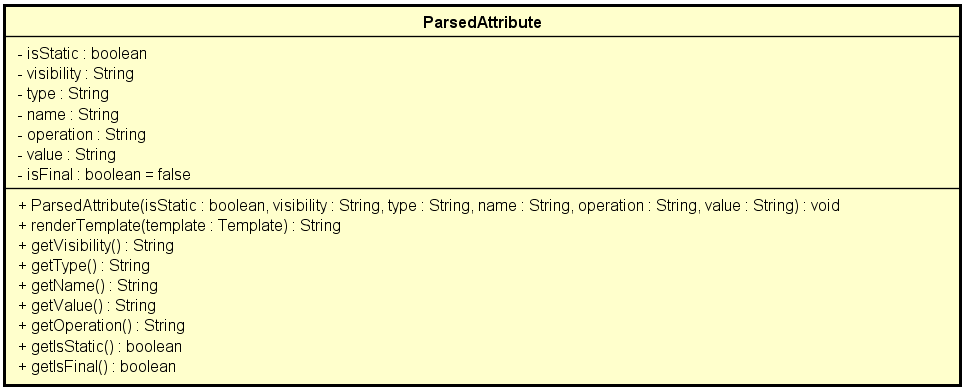
\includegraphics[scale=0.5,keepaspectratio]{img/server/ParsedAttribute.png}}
\caption{\nogloxy{swedesigner::server::project::ParsedAttribute}}
\end{figure}
\FloatBarrier
\begin{itemize}
\item \textbf{Descrizione}\\
questa classe rappresenta un singolo attributo, memorizzando il nome della variabile, la sua visibilità e il suo valore di default. Viene utilizzata anche per rappresentare i parametri dei metodi.
% Tuttavia, ciò non vale per attributi statici. 
% Nella \emph{Definizione_di_prodotto_v_1_0_0} [RIFERIMENTO] sarà esplicitata l'implementazione di dettaglio decisa.
\item \textbf{Utilizzo}\\
questa classe è usata da \texttt{ParsedMethod},  \texttt{ParsedClass} e \texttt{ParsedInterface} (le interfacce possono però contenere solo costanti di classe).
Questa classe implementa l'interfaccia \texttt{ParsedElement}.
Nota: Memorizzare il valore di questo attributo risulta superfluo, in quanto questo può essere impostato da un \texttt{ParsedAssignment}. 

\item \textbf{Relazioni con altre classi}:
\begin{itemize}
\item \textit{IN} \hyperref[\nogloxy{swedesigner::server::project::ParsedClass}]{\nogloxy{\texttt{ParsedClass}}}\\
questa classe estende la classe astratta \texttt{ParsedType}, imponendo al suo interno la presenza di una lista di \texttt{ParsedAttribute}. 
\item \textit{IN} \hyperref[\nogloxy{swedesigner::server::project::ParsedMethod}]{\nogloxy{\texttt{ParsedMethod}}}\\
questa classe rappresenta un metodo come insieme di istruzioni \texttt{ParsedIstruction} e un insieme di \texttt{ParsedAttribute} come parametri del metodo.
\item \textit{IN} \hyperref[\nogloxy{swedesigner::server::project::ParsedMethod}]{\nogloxy{\texttt{ParsedMethod}}}\\
questa classe rappresenta un metodo come insieme di istruzioni \texttt{ParsedIstruction} e un insieme di \texttt{ParsedAttribute} come parametri del metodo.
\item \textit{OUT} \hyperref[\nogloxy{swedesigner::server::project::ParsedElement}]{\nogloxy{\texttt{ParsedElement}}}\\
questa classe descrive il contratto di un elemento generico \texttt{Parsed}. Si specifica il metodo \texttt{RenderTemplate} che impone la necessità di implementarlo ad ogni classe sottostante.
\end{itemize}
\item \textbf{Attributi}:
\begin{itemize}
\item \nogloxy{\texttt{- isFinal: boolean}}
\\ Indica se l'oggetto ParsedAttribute è costante.
\item \nogloxy{\texttt{- isStatic: boolean}}
\\ Indica se il ParsedAttribute è un oggetto statico.
\item \nogloxy{\texttt{- name: String}}
\\ Indica il nome dell'oggetto ParsedAttribute.
\item \nogloxy{\texttt{- operation: String}}
\\ Indica l'operatore di assegnazione del valore iniziale dell'oggetto ParsedAttribute.
\item \nogloxy{\texttt{- type: String}}
\\ Indica il tipo dell'oggetto ParsedAttribute.
\item \nogloxy{\texttt{- value: String}}
\\ Indica il valore iniziale dell'oggetto ParsedAttribute.
\item \nogloxy{\texttt{- visibility: String}}
\\ Indica la visibilità dell'oggetto ParsedAttribute.
\end{itemize}
\item \textbf{Metodi}:
\begin{itemize}
\item \nogloxy{\texttt{+ getIsFinal(): boolean}}
\\ Ritorna informazioni relative alla natura costante di un oggetto ParsedAttribute.
\item \nogloxy{\texttt{+ getIsStatic(): boolean}}
\\ Ritorna informazioni riguardanti la staticità di un oggetto ParsedAttribute.
\item \nogloxy{\texttt{+ getName(): String}}
\\ Ritorna il nome di un oggetto ParsedAttribute.
\item \nogloxy{\texttt{+ getOperation(): String}}
\\ Ritorna l'operatore di assegnazione del valore iniziale di un oggetto ParsedAttribute.
\item \nogloxy{\texttt{+ getType(): String}}
\\ Ritorna il tipo di un oggetto ParsedAttribute.
\item \nogloxy{\texttt{+ getValue(): String}}
\\ Ritorna il valore iniziale di un oggetto ParsedAttribute.
\item \nogloxy{\texttt{+ getVisibility(): String}}
\\ Ritorna la visibilità di un oggetto ParsedAttribute.
\item \nogloxy{\texttt{+ ParsedAttribute(isStatic: boolean, visibility: String, type: String, name: String, operation: String, value: String)}}
\\ Costruisce un oggetto ParsedAttribute.
\\ \textbf{Parametri}:
\begin{itemize}
\item \nogloxy{\texttt{isStatic: boolean}}
\\ Indica se il ParsedAttribute che si sta creando è un oggetto statico.
\item \nogloxy{\texttt{visibility: String}}
\\ Indica la visibilità dell'oggetto ParsedAttribute che si sta creando.
\item \nogloxy{\texttt{type: String}}
\\ Indica il tipo dell'oggetto ParsedAttribute che si sta creando.
\item \nogloxy{\texttt{name: String}}
\\  Indica il nome dell'oggetto ParsedAttribute che si sta creando.
\item \nogloxy{\texttt{operation: String}}
\\ Indica l'operatore di assegnazione del valore iniziale dell'oggetto ParsedAttribute che si sta creando.
\item \nogloxy{\texttt{value: String}}
\\ Indica il valore iniziale dell'oggetto ParsedAttribute che si sta creando.
\end{itemize}
\item \nogloxy{\texttt{+ renderTemplate(template: Template): String}}
\\ Traduce l'oggetto ParsedAttribute in una stringa che rappresenta il codice di un particolare linguaggio di programmazione.
\\ \textbf{Parametri}:
\begin{itemize}
\item \nogloxy{\texttt{template: Template}}
\\ Riferimento alla particolare istanza di Template da utilizzare.
\end{itemize}
\end{itemize}
\end{itemize}

\subsubsubsection{\nogloxy{swedesigner::server::project::ParsedClass}}
\label{\nogloxy{swedesigner::server::project::ParsedClass}}
\begin{figure}[h]
\centering
\nogloxy{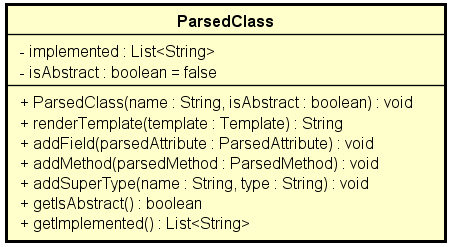
\includegraphics[scale=0.8,keepaspectratio]{img/server/ParsedClass.png}}
\caption{\nogloxy{swedesigner::server::project::ParsedClass}}
\end{figure}
\FloatBarrier
\begin{itemize}
\item \textbf{Descrizione}\\
questa classe estende la classe astratta \texttt{ParsedType}, imponendo al suo interno la presenza di una lista di \texttt{ParsedAttribute}. 
\item \textbf{Utilizzo}\\
questa classe è creata tramite la \texttt{ElementFactory} durante il parsing del progetto e inserita all'interno di \texttt{ParsedProgram}.
\item \textbf{Classi ereditate}:
\begin{itemize}
\item \hyperref[\nogloxy{swedesigner::server::project::ParsedType}]{\nogloxy{\texttt{ParsedType}}}
\end{itemize}
\item \textbf{Relazioni con altre classi}:
\begin{itemize}
\item \textit{IN} \hyperref[\nogloxy{swedesigner::server::project::ParsedException}]{\nogloxy{\texttt{ParsedException}}}\\
Questa classe rappresenta una eccezione che viene sollevata nel momento in cui viene identificata una illegalità nel parsing della stringa in formato .json
\item \textit{OUT} \hyperref[\nogloxy{swedesigner::server::project::ParsedAttribute}]{\nogloxy{\texttt{ParsedAttribute}}}\\
questa classe rappresenta un singolo attributo, memorizzando il nome della variabile, la sua visibilità e il suo valore di default. Viene utilizzata anche per rappresentare i parametri dei metodi.
% Tuttavia, ciò non vale per attributi statici. 
% Nella \emph{Definizione_di_prodotto_v_1_0_0} [RIFERIMENTO] sarà esplicitata l'implementazione di dettaglio decisa.
\item \textit{OUT} \hyperref[\nogloxy{swedesigner::server::project::ParsedMethod}]{\nogloxy{\texttt{ParsedMethod}}}\\
questa classe rappresenta un metodo come insieme di istruzioni \texttt{ParsedIstruction} e un insieme di \texttt{ParsedAttribute} come parametri del metodo.
\end{itemize}
\item \textbf{Attributi}:
\begin{itemize}
\item \nogloxy{\texttt{- implemented: List<String>}}
\\ Indica i nomi delle interfacce implementate.
\item \nogloxy{\texttt{- isAbstract: boolean}}
\\ Indica se l'oggetto ParsedClass è astratto o meno, ovvero se ha delle componenti che devono essere implementate.
\end{itemize}
\item \textbf{Metodi}:
\begin{itemize}
\item \nogloxy{\texttt{+ addField(parsedAttribute: ParsedAttribute): void}}
\\ Aggiunge all'oggetto ParsedClass un attributo rappresentato da un oggetto ParsedAttribute.
\\ \textbf{Parametri}:
\begin{itemize}
\item \nogloxy{\texttt{parsedAttribute: ParsedAttribute}}
\\ Indica il ParsedAttribute che deve essere aggiunto alla ParsedClass.
\end{itemize}
\item \nogloxy{\texttt{+ addMethod(parsedMethod: ParsedMethod): void}}
\\ Aggiunge ad un oggetto ParsedClass un metodo rappresentato da un oggetto ParsedMethod.
\\ \textbf{Parametri}:
\begin{itemize}
\item \nogloxy{\texttt{parsedMethod: ParsedMethod}}
\\ Indica il ParsedMethod che deve essere aggiunto alla ParsedClass.
\end{itemize}
\item \nogloxy{\texttt{+ addSupertype(name: String, type: String): void}}
\\ Aggiunge il nome di uno dei "supertipi" diretti dell'oggetto ParsedClass.
\\ \textbf{Parametri}:
\begin{itemize}
\item \nogloxy{\texttt{name: String}}
\\ Indica il nome del "supertipo" che deve essere implementato o esteso.
\item \nogloxy{\texttt{type: String}}
\\ Indica il tipo, classe o interfaccia, che deve essere rispettivamente esteso o implementato.
\end{itemize}
\item \nogloxy{\texttt{+ getImplemented(): List<String>}}
\\ Ritorna i nomi delle interfacce implementate.
\item \nogloxy{\texttt{+ getIsAbstract(): boolean}}
\\ Ritorna informazioni relative astrattezza dell'oggetto ParsedClass.
\item \nogloxy{\texttt{+ ParsedClass(name: String, isAbstract: boolean)}}
\\ Costruisce un oggetto ParsedClass.
\\ \textbf{Parametri}:
\begin{itemize}
\item \nogloxy{\texttt{name: String}}
\\ Rappresenta il nome del particolare oggetto ParsedClass che si sta creando.
\item \nogloxy{\texttt{isAbstract: boolean}}
\\ Indica se l'oggetto ParsedClass che si sta creando è astratto o meno.
\end{itemize}
\item \nogloxy{\texttt{+ renderTemplate(template: Template): String}}
\\ Traduce l'oggetto ParsedClass in una stringa che rappresenta il codice di un particolare linguaggio di programmazione.
\\ \textbf{Parametri}:
\begin{itemize}
\item \nogloxy{\texttt{template: Template}}
\\ Riferimento alla particolare istanza di Template da utilizzare.
\end{itemize}
\end{itemize}
\end{itemize}

\subsubsubsection{\nogloxy{swedesigner::server::project::ParsedCustom}}
\label{\nogloxy{swedesigner::server::project::ParsedCustom}}
\begin{figure}[h]
\centering
\nogloxy{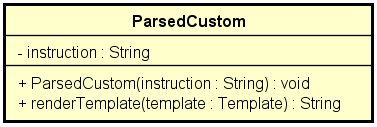
\includegraphics[scale=0.8,keepaspectratio]{img/server/ParsedCustom.png}}
\caption{\nogloxy{swedesigner::server::project::ParsedCustom}}
\end{figure}
\FloatBarrier
\begin{itemize}
\item \textbf{Descrizione}\\
questa classe descrive il comportamento di un blocco di codice custom, scritto nel linguaggio target.	
\item \textbf{Utilizzo}\\
dispone della possibilità di effettuare il render di un template in ingresso.
\item \textbf{Classi ereditate}:
\begin{itemize}
\item \hyperref[\nogloxy{swedesigner::server::project::ParsedInstruction}]{\nogloxy{\texttt{ParsedInstruction}}}
\end{itemize}
\item \textbf{Attributi}:
\begin{itemize}
\item \nogloxy{\texttt{- instruction: String}}
\\ Indica il codice inserito dall'utente in blocco custom.
\end{itemize}
\item \textbf{Metodi}:
\begin{itemize}
\item \nogloxy{\texttt{+ ParsedCustom(instruction: String)}}
\\ Costruisce un oggetto ParsedCustom.
\\ \textbf{Parametri}:
\begin{itemize}
\item \nogloxy{\texttt{instruction: String}}
\\ Indica l'insieme di istruzioni inserite dall'utente.
\end{itemize}
\item \nogloxy{\texttt{+ renderTemplate(template: Template): String}}
\\ Traduce l'oggetto ParsedCustom in una stringa che rappresenta il codice di un particolare linguaggio di programmazione.
\\ \textbf{Parametri}:
\begin{itemize}
\item \nogloxy{\texttt{template: Template}}
\\ Riferimento alla particolare istanza di Template da utilizzare.
\end{itemize}
\end{itemize}
\end{itemize}

\subsubsubsection{\nogloxy{swedesigner::server::project::ParsedElement}}
\label{\nogloxy{swedesigner::server::project::ParsedElement}}
\begin{figure}[h]
\centering
\nogloxy{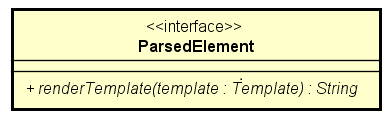
\includegraphics[scale=0.8,keepaspectratio]{img/server/ParsedElement.png}}
\caption{\nogloxy{swedesigner::server::project::ParsedElement}}
\end{figure}
\FloatBarrier
\begin{itemize}
\item \textbf{Descrizione}\\
questa classe descrive il contratto di un elemento generico \texttt{Parsed}. Si specifica il metodo \texttt{RenderTemplate} che impone la necessità di implementarlo ad ogni classe sottostante.
\item \textbf{Utilizzo}\\
questa interfaccia è usata da \texttt{ElementFactory}, la quale fornisce un metodo per creare nuovi elementi secondo il design pattern Factory. %[RIFERIMENTO AD APPENDICE].
\item \textbf{Sottoclassi}:
\begin{itemize}
\item \hyperref[\nogloxy{swedesigner::server::project::ParsedMethod}]{\nogloxy{\texttt{ParsedMethod}}}
\end{itemize}
\item \textbf{Relazioni con altre classi}:
\begin{itemize}
\item \textit{IN} \hyperref[\nogloxy{swedesigner::server::generator::Generator}]{\nogloxy{\texttt{Generator}}}\\
questa interfaccia si occupa di fornire un oggetto \texttt{Generator} generico a chi lo richiede in modo da poter rendere entensibile il sistema aggiungendo un'implementazione concreta del generator del linguaggio target desiderato.
\item \textit{IN} \hyperref[\nogloxy{swedesigner::server::project::ParsedAttribute}]{\nogloxy{\texttt{ParsedAttribute}}}\\
questa classe rappresenta un singolo attributo, memorizzando il nome della variabile, la sua visibilità e il suo valore di default. Viene utilizzata anche per rappresentare i parametri dei metodi.
% Tuttavia, ciò non vale per attributi statici. 
% Nella \emph{Definizione_di_prodotto_v_1_0_0} [RIFERIMENTO] sarà esplicitata l'implementazione di dettaglio decisa.
\item \textit{IN} \hyperref[\nogloxy{swedesigner::server::project::ParsedInstruction}]{\nogloxy{\texttt{ParsedInstruction}}}\\
questa classe astratta rappresenta la singola istruzione contenuta all'interno di un metodo. Essa è estesa dalle istruzioni specifiche (e.g. \texttt{ParsedIf}, \texttt{ParsedWhile}, etc.)
\item \textit{IN} \hyperref[\nogloxy{swedesigner::server::project::ParsedMethod}]{\nogloxy{\texttt{ParsedMethod}}}\\
questa classe rappresenta un metodo come insieme di istruzioni \texttt{ParsedIstruction} e un insieme di \texttt{ParsedAttribute} come parametri del metodo.
\item \textit{IN} \hyperref[\nogloxy{swedesigner::server::project::ParsedMethod}]{\nogloxy{\texttt{ParsedMethod}}}\\
questa classe rappresenta un metodo come insieme di istruzioni \texttt{ParsedIstruction} e un insieme di \texttt{ParsedAttribute} come parametri del metodo.
\item \textit{IN} \hyperref[\nogloxy{swedesigner::server::project::ParsedType}]{\nogloxy{\texttt{ParsedType}}}\\
questa classe astratta definisce un contratto comune tra le classi \texttt{ParsedInterface} e \texttt{ParsedClass}. 
\end{itemize}
\item \textbf{Metodi}:
\begin{itemize}
\item \nogloxy{\texttt{+ renderTemplate(template: Template): String}}
\\ Traduce l'oggetto ParsedElement in una stringa che rappresenta il codice di un particolare linguaggio di programmazione.
\\ \textbf{Parametri}:
\begin{itemize}
\item \nogloxy{\texttt{template: Template}}
\\ Riferimento alla particolare istanza di Template da utilizzare.
\end{itemize}
\end{itemize}
\end{itemize}

\subsubsubsection{\nogloxy{swedesigner::server::project::ParsedElse}}
\label{\nogloxy{swedesigner::server::project::ParsedElse}}
\begin{figure}[h]
\centering
\nogloxy{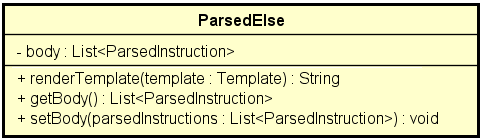
\includegraphics[scale=0.8,keepaspectratio]{img/server/ParsedElse.png}}
\caption{\nogloxy{swedesigner::server::project::ParsedElse}}
\end{figure}
\FloatBarrier
\begin{itemize}
\item \textbf{Descrizione}\\
questa classe descrive il comportamento di un blocco \texttt{else}.
\item \textbf{Utilizzo}\\
dispone della possibilità di effettuare il render di un template in ingresso.
\item \textbf{Classi ereditate}:
\begin{itemize}
\item \hyperref[\nogloxy{swedesigner::server::project::ParsedInstruction}]{\nogloxy{\texttt{ParsedInstruction}}}
\end{itemize}
\item \textbf{Attributi}:
\begin{itemize}
\item \nogloxy{\texttt{- body: List<ParsedInstruction>}}
\\ Indica l'insieme di istruzioni contenute nel corpo del corrispondente oggetto ParsedElse.
\end{itemize}
\item \textbf{Metodi}:
\begin{itemize}
\item \nogloxy{\texttt{+ getBody(): List<ParsedInstruction>}}
\\ Ritorna l'insieme di istruzioni che compongono il corpo del relativo oggetto ParsedElse.
\item \nogloxy{\texttt{+ renderTemplate(template: Template): String}}
\\ Traduce l'oggetto ParsedElse in una stringa che rappresenta il codice di un particolare linguaggio di programmazione.
\\ \textbf{Parametri}:
\begin{itemize}
\item \nogloxy{\texttt{template: Template}}
\\ Riferimento alla particolare istanza di Template da utilizzare.
\end{itemize}
\item \nogloxy{\texttt{+ setBody(parsedInstructions: List<ParsedInstruction>): void}}
\\ Inserisce nel campo dati body del ParsedElse un insieme di ParsedInstruction, ossia inserisce il corpo all'interno del body dell'istruzione \emph{else}.
\\ \textbf{Parametri}:
\begin{itemize}
\item \nogloxy{\texttt{parsedInstructions: List<ParsedInstruction>}}
\\ Rappresenta l'insieme di istruzioni da inserire nel corpo del corrispondente oggetto ParsedElse.
\end{itemize}
\end{itemize}
\end{itemize}

\subsubsubsection{\nogloxy{swedesigner::server::project::ParsedException}}
\label{\nogloxy{swedesigner::server::project::ParsedException}}
\begin{figure}[h]
\centering
\nogloxy{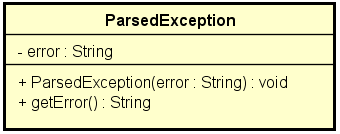
\includegraphics[scale=0.8,keepaspectratio]{img/server/ParsedException.png}}
\caption{\nogloxy{swedesigner::server::project::ParsedException}}
\end{figure}
\FloatBarrier
\begin{itemize}
\item \textbf{Descrizione}\\
Questa classe rappresenta una eccezione che viene sollevata nel momento in cui viene identificata una illegalità nel parsing della stringa in formato .json
\item \textbf{Utilizzo}\\
\texttt{ParsedInterface} solleva un'eccezione nel caso in cui venga identificata una illegalità nel parsing di una interfaccia. Inoltre \texttt{ParsedClass} solleva tale eccezione nel caso venga identificata una illegalità nel parsing di una classe.
\item \textbf{Relazioni con altre classi}:
\begin{itemize}
\item \textit{OUT} \hyperref[\nogloxy{swedesigner::server::project::ParsedClass}]{\nogloxy{\texttt{ParsedClass}}}\\
questa classe estende la classe astratta \texttt{ParsedType}, imponendo al suo interno la presenza di una lista di \texttt{ParsedAttribute}. 
\item \textit{OUT} \hyperref[\nogloxy{swedesigner::server::project::ParsedInterface}]{\nogloxy{\texttt{ParsedInterface}}}\\
questa classe estende la classe astratta \textt{ParsedType} ed ha bisogno soltanto della firma dei metodi essendo una classe che contiene informazioni riguardo un'interfaccia pura.
\end{itemize}
\item \textbf{Attributi}:
\begin{itemize}
\item \nogloxy{\texttt{- error: String}}
\\ Rappresenta la descrizione testuale dell'errore rilevato in fase di parsing.
\end{itemize}
\item \textbf{Metodi}:
\begin{itemize}
\item \nogloxy{\texttt{+ getError(): String}}
\\ Ritorna la descrizione testuale di un errore rilevato in fase di parsing.
\item \nogloxy{\texttt{+ ParsedException(error: String)}}
\\ Costruisce un oggetto ParsedException.
\\ \textbf{Parametri}:
\begin{itemize}
\item \nogloxy{\texttt{error: String}}
\\ Rappresenta il contenuto di un particolare errore.
\end{itemize}
\end{itemize}
\end{itemize}

\subsubsubsection{\nogloxy{swedesigner::server::project::ParsedFor}}
\label{\nogloxy{swedesigner::server::project::ParsedFor}}
\begin{figure}[h]
\centering
\nogloxy{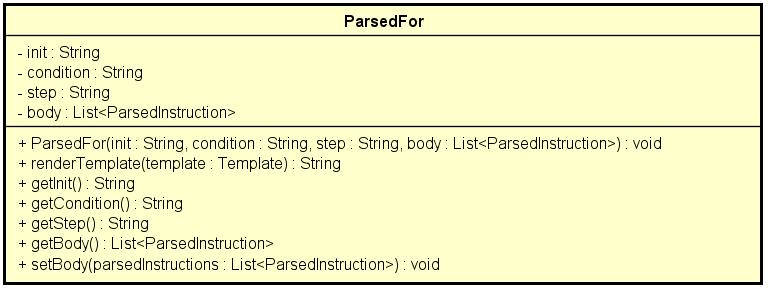
\includegraphics[scale=0.6,keepaspectratio]{img/server/ParsedFor.png}}
\caption{\nogloxy{swedesigner::server::project::ParsedFor}}
\end{figure}
\FloatBarrier
\begin{itemize}
\item \textbf{Descrizione}\\
questa classe descrive il comportamento di un blocco \texttt{for}.
\item \textbf{Utilizzo}\\
dispone della possibilità di effettuare il render di un template in ingresso.
\item \textbf{Classi ereditate}:
\begin{itemize}
\item \hyperref[\nogloxy{swedesigner::server::project::ParsedInstruction}]{\nogloxy{\texttt{ParsedInstruction}}}
\end{itemize}
\item \textbf{Attributi}:
\begin{itemize}
\item \nogloxy{\texttt{- body: List<ParsedInstruction>}}
\\ Indica l'insieme di istruzioni contenute nel corpo del corrispondente oggetto ParsedFor.
\item \nogloxy{\texttt{- condition: String}}
\\ Indica la condizione del corrispondente oggetto ParsedFor.
\item \nogloxy{\texttt{- init: String}}
\\ Indica l'istruzione di inizializzazione del corrispondente oggetto ParsedFor.
\item \nogloxy{\texttt{- step: String}}
\\ Indica il passo di incremento o decremento del corrispondente oggetto ParsedFor.
\end{itemize}
\item \textbf{Metodi}:
\begin{itemize}
\item \nogloxy{\texttt{+ getBody(): List<ParsedInstruction>}}
\\ Ritorna l'insieme di istruzioni contenute nel corpo di un oggetto ParsedFor.
\item \nogloxy{\texttt{+ getCondition(): String}}
\\ Ritorna la condizione di un oggetto ParsedFor.
\item \nogloxy{\texttt{+ getInit(): String}}
\\ Ritorna l'istruzione di inizializzazione dell'oggetto ParsedFor.
\item \nogloxy{\texttt{+ getStep(): String}}
\\ Ritorna il passo di incremento o decremento di un oggetto ParsedFor.
\item \nogloxy{\texttt{+ ParsedFor(init: String, condition: String, step: String)}}
\\ Costruisce un oggetto ParsedFor.
\\ \textbf{Parametri}:
\begin{itemize}
\item \nogloxy{\texttt{init: String}}
\\ Rappresenta l'istruzione di inizializzazione del particolare oggetto ParsedFor che si sta creando.
\item \nogloxy{\texttt{condition: String}}
\\ Rappresenta la condizione del particolare oggetto ParsedFor che si sta creando.

\item \nogloxy{\texttt{step: String}}
\\ Rapprensenta il passo di incremento o decremento del particolare oggetto ParsedFor che si sta creando.
\end{itemize}
\item \nogloxy{\texttt{+ renderTemplate(template: Template): String}}
\\ Traduce l'oggetto ParsedFor in una stringa che rappresenta il codice di un particolare linguaggio di programmazione.
\\ \textbf{Parametri}:
\begin{itemize}
\item \nogloxy{\texttt{template: Template}}
\\ Riferimento alla particolare istanza di Template da utilizzare.
\end{itemize}
\item \nogloxy{\texttt{+ setBody(parsedInstructions: List<ParsedInstruction>): void}}
\\ Permette di assegnare un insieme di istruzioni al corpo di un oggetto ParsedFor.
\\ \textbf{Parametri}:
\begin{itemize}
\item \nogloxy{\texttt{parsedInstructions: List<ParsedInstruction>}}
\\ Rappresenta l'insieme di istruzioni da inserire nel corpo del corrispondente oggetto ParsedFor.
\end{itemize}
\end{itemize}
\end{itemize}

\subsubsubsection{\nogloxy{swedesigner::server::project::ParsedIf}}
\label{\nogloxy{swedesigner::server::project::ParsedIf}}
\begin{figure}[h]
\centering
\nogloxy{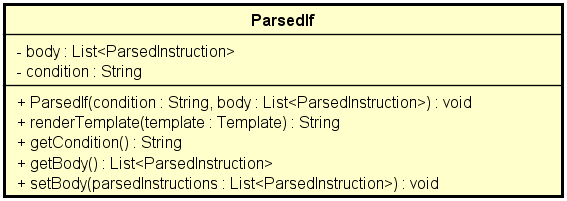
\includegraphics[scale=0.8,keepaspectratio]{img/server/ParsedIf.png}}
\caption{\nogloxy{swedesigner::server::project::ParsedIf}}
\end{figure}
\FloatBarrier
\begin{itemize}
\item \textbf{Descrizione}\\
questa classe descrive il comportamento di un blocco \texttt{if}.
\item \textbf{Utilizzo}\\
dispone della possibilità di effettuare il render di un template in ingresso.
\item \textbf{Classi ereditate}:
\begin{itemize}
\item \hyperref[\nogloxy{swedesigner::server::project::ParsedInstruction}]{\nogloxy{\texttt{ParsedInstruction}}}
\end{itemize}
\item \textbf{Attributi}:
\begin{itemize}
\item \nogloxy{\texttt{- body: List<ParsedInstruction>}}
\\ Indica l'insieme di istruzioni contenute nel corpo del corrispondente oggetto ParsedIf.
\item \nogloxy{\texttt{- condition: String}}
\\ Indica la condizione del corrispondente oggetto ParsedIf.
\end{itemize}
\item \textbf{Metodi}:
\begin{itemize}
\item \nogloxy{\texttt{+ getBody(): List<ParsedInstruction>}}
\\ Ritorna l'insieme di istruzioni contenute nel corpo di un oggetto ParsedIf.
\item \nogloxy{\texttt{+ getCondition(): String}}
\\ Ritorna la condizione di un oggetto ParsedIf.
\item \nogloxy{\texttt{+ ParsedIf(condition: String)}}
\\ Costruisce un oggetto ParsedIf.
\\ \textbf{Parametri}:
\begin{itemize}
\item \nogloxy{\texttt{condition: String}}
\\ Rappresenta la condizione del particolare oggetto ParsedIf che si sta creando.
\end{itemize}
\item \nogloxy{\texttt{+ renderTemplate(template: Template): String}}
\\ Traduce l'oggetto ParsedIf in una stringa che rappresenta il codice di un particolare linguaggio di programmazione.
\\ \textbf{Parametri}:
\begin{itemize}
\item \nogloxy{\texttt{template: Template}}
\\ Riferimento alla particolare istanza di Template da utilizzare.
\end{itemize}
\item \nogloxy{\texttt{+ setBody(parsedInstructions: List<ParsedInstruction>): void}}
\\ Inserisce nel campo dati body del ParsedIf un insieme di ParsedInstruction, ossia inserisce il corpo all'interno del body dell'istruzione \emph{if}.
\\ \textbf{Parametri}:
\begin{itemize}
\item \nogloxy{\texttt{parsedInstructions: List<ParsedInstruction>}}
\\ Indica l'insieme di istruzioni da inserire nel corpo del corrispondente oggetto ParsedIf.
\end{itemize}
\end{itemize}
\end{itemize}

\subsubsubsection{\nogloxy{swedesigner::server::project::ParsedInstruction}}
\label{\nogloxy{swedesigner::server::project::ParsedInstruction}}
\begin{figure}[h]
\centering
\nogloxy{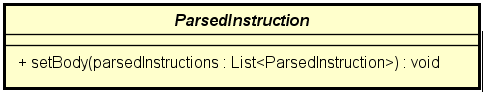
\includegraphics[scale=0.8,keepaspectratio]{img/server/ParsedInstruction.png}}
\caption{\nogloxy{swedesigner::server::project::ParsedInstruction}}
\end{figure}
\FloatBarrier
\begin{itemize}
\item \textbf{Descrizione}\\
questa classe astratta rappresenta la singola istruzione contenuta all'interno di un metodo. Essa è estesa dalle istruzioni specifiche (e.g. \texttt{ParsedIf}, \texttt{ParsedWhile}, etc.)
\item \textbf{Utilizzo}\\
questa classe implementa l'interfaccia \texttt{ParsedElement}.
\item \textbf{Sottoclassi}:
\begin{itemize}
\item \hyperref[\nogloxy{swedesigner::server::project::ParsedCustom}]{\nogloxy{\texttt{ParsedCustom}}}
\item \hyperref[\nogloxy{swedesigner::server::project::ParsedElse}]{\nogloxy{\texttt{ParsedElse}}}
\item \hyperref[\nogloxy{swedesigner::server::project::ParsedFor}]{\nogloxy{\texttt{ParsedFor}}}
\item \hyperref[\nogloxy{swedesigner::server::project::ParsedIf}]{\nogloxy{\texttt{ParsedIf}}}
\item \hyperref[\nogloxy{swedesigner::server::project::ParsedReturn}]{\nogloxy{\texttt{ParsedReturn}}}
\item \hyperref[\nogloxy{swedesigner::server::project::ParsedStatement}]{\nogloxy{\texttt{ParsedStatement}}}
\item \hyperref[\nogloxy{swedesigner::server::project::ParsedWhile}]{\nogloxy{\texttt{ParsedWhile}}}
\end{itemize}
\item \textbf{Relazioni con altre classi}:
\begin{itemize}
\item \textit{IN} \hyperref[\nogloxy{swedesigner::server::project::ParsedMethod}]{\nogloxy{\texttt{ParsedMethod}}}\\
questa classe rappresenta un metodo come insieme di istruzioni \texttt{ParsedIstruction} e un insieme di \texttt{ParsedAttribute} come parametri del metodo.
\item \textit{IN} \hyperref[\nogloxy{swedesigner::server::project::ParsedMethod}]{\nogloxy{\texttt{ParsedMethod}}}\\
questa classe rappresenta un metodo come insieme di istruzioni \texttt{ParsedIstruction} e un insieme di \texttt{ParsedAttribute} come parametri del metodo.
\item \textit{OUT} \hyperref[\nogloxy{swedesigner::server::project::ParsedElement}]{\nogloxy{\texttt{ParsedElement}}}\\
questa classe descrive il contratto di un elemento generico \texttt{Parsed}. Si specifica il metodo \texttt{RenderTemplate} che impone la necessità di implementarlo ad ogni classe sottostante.
\end{itemize}
\item \textbf{Metodi}:
\begin{itemize}
\item \nogloxy{\texttt{+ setBody(parsedInstructions: List<ParsedInstruction>): void}}
\\ Permette di assegnare un insieme di istruzioni al corpo di un oggetto ParsedInstruction.
\\ \textbf{Parametri}:
\begin{itemize}
\item \nogloxy{\texttt{parsedInstructions: List<ParsedInstruction>}}
\\ Rappresenta l'insieme di istruzioni da inserire nel corpo di una particolare ParsedInstruction.
\end{itemize}
\end{itemize}
\end{itemize}

\subsubsubsection{\nogloxy{swedesigner::server::project::ParsedInterface}}
\label{\nogloxy{swedesigner::server::project::ParsedInterface}}
\begin{figure}[h]
\centering
\nogloxy{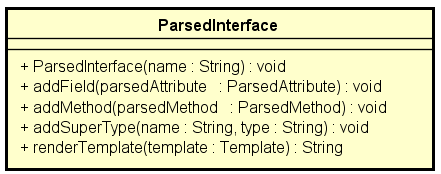
\includegraphics[scale=0.8,keepaspectratio]{img/server/ParsedInterface.png}}
\caption{\nogloxy{swedesigner::server::project::ParsedInterface}}
\end{figure}
\FloatBarrier
\begin{itemize}
\item \textbf{Descrizione}\\
questa classe estende la classe astratta \textt{ParsedType} ed ha bisogno soltanto della firma dei metodi essendo una classe che contiene informazioni riguardo un'interfaccia pura.
\item \textbf{Utilizzo}\\
questa classe è creata tramite la \texttt{ElementFactory} durante il parsing del progetto e inserita all'interno di \texttt{ParsedProgram}.
\item \textbf{Classi ereditate}:
\begin{itemize}
\item \hyperref[\nogloxy{swedesigner::server::project::ParsedType}]{\nogloxy{\texttt{ParsedType}}}
\end{itemize}
\item \textbf{Relazioni con altre classi}:
\begin{itemize}
\item \textit{IN} \hyperref[\nogloxy{swedesigner::server::project::ParsedException}]{\nogloxy{\texttt{ParsedException}}}\\
Questa classe rappresenta una eccezione che viene sollevata nel momento in cui viene identificata una illegalità nel parsing della stringa in formato .json
\item \textit{OUT} \hyperref[\nogloxy{swedesigner::server::project::ParsedMethod}]{\nogloxy{\texttt{ParsedMethod}}}\\
questa classe rappresenta un metodo come insieme di istruzioni \texttt{ParsedIstruction} e un insieme di \texttt{ParsedAttribute} come parametri del metodo.
\end{itemize}
\item \textbf{Metodi}:
\begin{itemize}
\item \nogloxy{\texttt{+ addField(parsedAttribute: ParsedAttribute): void}}
\\ Aggiunge all'oggetto ParsedInterface un campo dati rappresentato da un oggetto ParsedAttribute.
\\ \textbf{Parametri}:
\begin{itemize}
\item \nogloxy{\texttt{parsedAttribute: ParsedAttribute}}
\\ Rappresenta un campo dati in forma di oggetto ParsedAttribute.
\end{itemize}
\item \nogloxy{\texttt{+ addMethod(parsedMethod: ParsedMethod): void}}
\\ Aggiunge ad un oggetto ParsedInterface un metodo rappresentato da un oggetto ParsedMethod.
\\ \textbf{Parametri}:
\begin{itemize}
\item \nogloxy{\texttt{parsedMethod: ParsedMethod}}
\\ Rappresenta un metodo in forma di oggetto ParsedMethod.
\end{itemize}
\item \nogloxy{\texttt{+ addSupertype(name: String, type: String): void}}
\\ Aggiunge il nome di uno dei "supertipi" diretti dell'oggetto ParsedInterface.
\\ \textbf{Parametri}:
\begin{itemize}
\item \nogloxy{\texttt{name: String}}
\\ Rappresenta il nome del "supertipo" che deve essere esteso.
\item \nogloxy{\texttt{type: String}}
\\ Indica il supertipo tipo che deve essere esteso.
\end{itemize}
\item \nogloxy{\texttt{+ ParsedInterface(name: String)}}
\\ Costruisce un oggetto ParsedInterface.
\\ \textbf{Parametri}:
\begin{itemize}
\item \nogloxy{\texttt{name: String}}
\\ Rappresenta il nome del particolare oggetto ParsedInterface che si sta creando.
\end{itemize}
\item \nogloxy{\texttt{+ renderTemplate(template: Template): String}}
\\ Traduce l'oggetto ParsedInterface in una stringa che rappresenta il codice di un particolare linguaggio di programmazione.
\\ \textbf{Parametri}:
\begin{itemize}
\item \nogloxy{\texttt{template: Template}}
\\ Riferimento alla particolare istanza di Template da utilizzare.
\end{itemize}
\end{itemize}
\end{itemize}

\subsubsubsection{\nogloxy{swedesigner::server::project::ParsedMethod}}
\label{\nogloxy{swedesigner::server::project::ParsedMethod}}
\begin{figure}[h]
\centering
\nogloxy{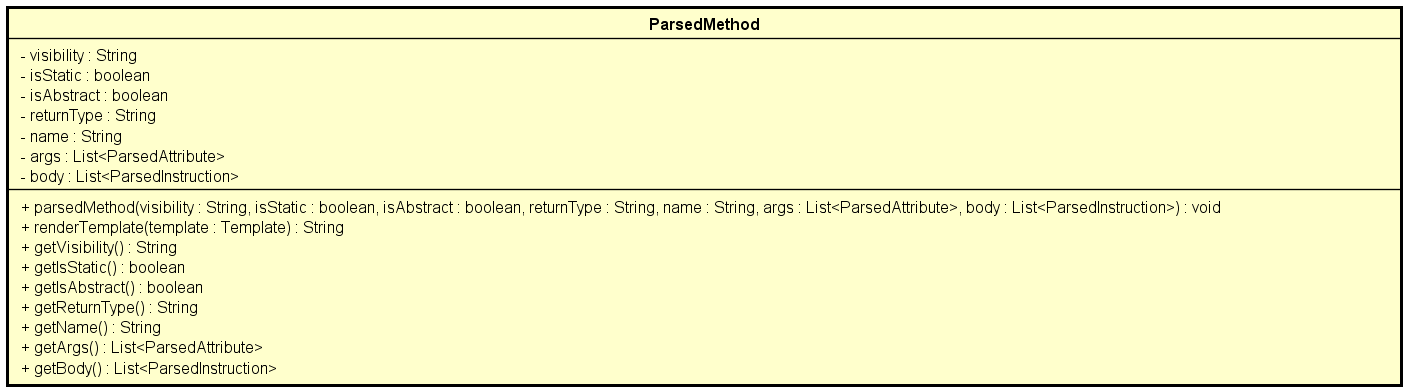
\includegraphics[scale=0.5,keepaspectratio]{img/server/ParsedMethod.png}}
\caption{\nogloxy{swedesigner::server::project::ParsedMethod}}
\end{figure}
\FloatBarrier
\begin{itemize}
\item \textbf{Descrizione}\\
questa classe rappresenta un metodo come insieme di istruzioni \texttt{ParsedIstruction} e un insieme di \texttt{ParsedAttribute} come parametri del metodo.
\item \textbf{Utilizzo}\\
questa classe è usata da \texttt{ParsedType} come descritto in precedenza. La classe inoltre implementa l'interfaccia \texttt{ParsedElement}.
\item \textbf{Classi ereditate}:
\begin{itemize}
\item \hyperref[\nogloxy{swedesigner::server::project::ParsedElement}]{\nogloxy{\texttt{ParsedElement}}}
\end{itemize}
\item \textbf{Relazioni con altre classi}:
\begin{itemize}
\item \textit{IN} \hyperref[\nogloxy{swedesigner::server::project::ParsedClass}]{\nogloxy{\texttt{ParsedClass}}}\\
questa classe estende la classe astratta \texttt{ParsedType}, imponendo al suo interno la presenza di una lista di \texttt{ParsedAttribute}. 
\item \textit{IN} \hyperref[\nogloxy{swedesigner::server::project::ParsedInterface}]{\nogloxy{\texttt{ParsedInterface}}}\\
questa classe estende la classe astratta \textt{ParsedType} ed ha bisogno soltanto della firma dei metodi essendo una classe che contiene informazioni riguardo un'interfaccia pura.
\item \textit{IN} \hyperref[\nogloxy{swedesigner::server::project::ParsedType}]{\nogloxy{\texttt{ParsedType}}}\\
questa classe astratta definisce un contratto comune tra le classi \texttt{ParsedInterface} e \texttt{ParsedClass}. 
\item \textit{OUT} \hyperref[\nogloxy{swedesigner::server::project::ParsedAttribute}]{\nogloxy{\texttt{ParsedAttribute}}}\\
questa classe rappresenta un singolo attributo, memorizzando il nome della variabile, la sua visibilità e il suo valore di default. Viene utilizzata anche per rappresentare i parametri dei metodi.
% Tuttavia, ciò non vale per attributi statici. 
% Nella \emph{Definizione_di_prodotto_v_1_0_0} [RIFERIMENTO] sarà esplicitata l'implementazione di dettaglio decisa.
\item \textit{OUT} \hyperref[\nogloxy{swedesigner::server::project::ParsedAttribute}]{\nogloxy{\texttt{ParsedAttribute}}}\\
questa classe rappresenta un singolo attributo, memorizzando il nome della variabile, la sua visibilità e il suo valore di default. Viene utilizzata anche per rappresentare i parametri dei metodi.
% Tuttavia, ciò non vale per attributi statici. 
% Nella \emph{Definizione_di_prodotto_v_1_0_0} [RIFERIMENTO] sarà esplicitata l'implementazione di dettaglio decisa.
\item \textit{OUT} \hyperref[\nogloxy{swedesigner::server::project::ParsedElement}]{\nogloxy{\texttt{ParsedElement}}}\\
questa classe descrive il contratto di un elemento generico \texttt{Parsed}. Si specifica il metodo \texttt{RenderTemplate} che impone la necessità di implementarlo ad ogni classe sottostante.
\item \textit{OUT} \hyperref[\nogloxy{swedesigner::server::project::ParsedElement}]{\nogloxy{\texttt{ParsedElement}}}\\
questa classe descrive il contratto di un elemento generico \texttt{Parsed}. Si specifica il metodo \texttt{RenderTemplate} che impone la necessità di implementarlo ad ogni classe sottostante.
\item \textit{OUT} \hyperref[\nogloxy{swedesigner::server::project::ParsedInstruction}]{\nogloxy{\texttt{ParsedInstruction}}}\\
questa classe astratta rappresenta la singola istruzione contenuta all'interno di un metodo. Essa è estesa dalle istruzioni specifiche (e.g. \texttt{ParsedIf}, \texttt{ParsedWhile}, etc.)
\item \textit{OUT} \hyperref[\nogloxy{swedesigner::server::project::ParsedInstruction}]{\nogloxy{\texttt{ParsedInstruction}}}\\
questa classe astratta rappresenta la singola istruzione contenuta all'interno di un metodo. Essa è estesa dalle istruzioni specifiche (e.g. \texttt{ParsedIf}, \texttt{ParsedWhile}, etc.)
\end{itemize}
\item \textbf{Attributi}:
\begin{itemize}
\item \nogloxy{\texttt{- args: List<ParsedAttribute>}}
\\ Indica l'insieme di ParsedAttribute che rappresentano i parametri di un ParsedMethod.
\item \nogloxy{\texttt{- body: List<ParsedInstruction>}}
\\ Indica l'insieme di istruzioni che compongono il corpo del relativo oggetto ParsedMethod.
\item \nogloxy{\texttt{- isAbstract: boolean}}
\\ Indica se il ParsedMethod rappresenta un metodo astratto o meno.
\item \nogloxy{\texttt{- isStatic: boolean}}
\\ Indica se il ParsedMethod rappresenta un metodo statico o meno.
\item \nogloxy{\texttt{- name: String}}
\\ Indica il nome dell'oggetto ParsedMethod.
\item \nogloxy{\texttt{- returnType: String}}
\\ Indica il tipo di ritorno di un oggetto ParsedMethod.
\item \nogloxy{\texttt{- visibility: String}}
\\ Indica la visibilità dell'oggetto ParsedMethod.
\end{itemize}
\item \textbf{Metodi}:
\begin{itemize}
\item \nogloxy{\texttt{+ getArgs(): List<ParsedAttribute>}}
\\ Ritorna l'insieme di ParsedAttribute che rappresentano i parametri di un ParsedMethod.
\item \nogloxy{\texttt{+ getBody(): List<ParsedInstruction>}}
\\ Ritorna l'insieme di istruzioni che compongono il corpo del relativo oggetto ParsedMethod.
\item \nogloxy{\texttt{+ getIsAbstract(): boolean}}
\\ Indica se l'oggetto ParsedMethod è astratto o meno.
\item \nogloxy{\texttt{+ getIsStatic(): boolean}}
\\ Ritorna informazioni riguardanti la staticità di un oggetto ParsedMethod.
\item \nogloxy{\texttt{+ getName(): String}}
\\ Ritorna il nome di un oggetto ParsedMethod.
\item \nogloxy{\texttt{+ getReturnType(): String}}
\\ Ritorna il tipo di ritorno di un oggetto ParsedMethod.
\item \nogloxy{\texttt{+ getVisibility(): String}}
\\ Ritorna la visibilità di un oggetto ParsedMethod.
\item \nogloxy{\texttt{+ ParsedMethod(visibility: String, isStatic: boolean, isAbstract: boolean, returnType: String, args: List<ParsedAttribute>, body: List<ParsedInstruction>, name: String)}}
\\ Costruisce un oggetto ParsedMethod.
\\ \textbf{Parametri}:
\begin{itemize}
\item \nogloxy{\texttt{visibility: String}}
\\ Rappresenta la visibilità dell'oggetto ParsedMethod che si sta creando.
\item \nogloxy{\texttt{isStatic: boolean}}
\\ Indica se il ParsedMethod che si sta creando rappresenterà un metodo statico o meno.
\item \nogloxy{\texttt{isAbstract: boolean}}
\\ Indica se il ParsedMethod che si sta creando rappresenterà un metodo astratto o meno.
\item \nogloxy{\texttt{returnType: String}}
\\ Indica il tipo di ritorno dell'oggetto ParsedMethod che si sta creando.
\item \nogloxy{\texttt{args: List<ParsedAttribute>}}
\\ Indica l'insieme di ParsedAttribute che rappresenteranno i parametri del ParsedMethod che si sta creando.
\item \nogloxy{\texttt{body: List<ParsedInstruction>}}
\\ Indica l'insieme di istruzioni che comporranno il corpo del relativo oggetto ParsedMethod che si sta creando.
\item \nogloxy{\texttt{name: String}}
\\ Indica il nome dell'oggetto ParsedMethod che si sta creando.
\end{itemize}
\item \nogloxy{\texttt{+ renderTemplate(template: Tempate): String}}
\\ Traduce l'oggetto ParsedMethod in una stringa che rappresenta il codice di un particolare linguaggio di programmazione.
\\ \textbf{Parametri}:
\begin{itemize}
\item \nogloxy{\texttt{template: Tempate}}
\\ Riferimento alla particolare istanza di Template da utilizzare.
\end{itemize}
\end{itemize}
\end{itemize}

\subsubsubsection{\nogloxy{swedesigner::server::project::ParsedProgram}}
\label{\nogloxy{swedesigner::server::project::ParsedProgram}}
\begin{figure}[h]
\centering
\nogloxy{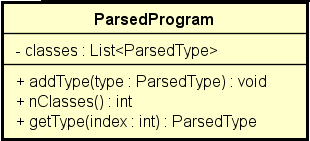
\includegraphics[scale=0.8,keepaspectratio]{img/server/ParsedProgram.png}}
\caption{\nogloxy{swedesigner::server::project::ParsedProgram}}
\end{figure}
\FloatBarrier
\begin{itemize}
\item \textbf{Descrizione}\\
questa classe rappresenta l'entità che possiede al suo interno tutte le componenti di un progetto. Essa possiede più \texttt{ParsedType}.
\item \textbf{Utilizzo}\\
La classe \texttt{Parser} ha una dipendenza verso questo elemento: essa infatti ne crea una e la ritorna al controller, il quale la passerà alla classe \texttt{Generator}.
\item \textbf{Relazioni con altre classi}:
\begin{itemize}
\item \textit{IN} \hyperref[\nogloxy{swedesigner::server::parser::Parser}]{\nogloxy{\texttt{Parser}}}\\
questa classe si occupa di elaborare il file JSON proveniente dal client e di creare da esso un oggetto Java \texttt{ParsedProgram} strutturato in modo da poter essere facilmente convertito in codice.
\item \textit{OUT} \hyperref[\nogloxy{swedesigner::server::project::ParsedType}]{\nogloxy{\texttt{ParsedType}}}\\
questa classe astratta definisce un contratto comune tra le classi \texttt{ParsedInterface} e \texttt{ParsedClass}. 
\end{itemize}
\item \textbf{Attributi}:
\begin{itemize}
\item \nogloxy{\texttt{- classes: List<ParsedType>}}
\\ Indica l'insieme di classi ed interfacce, sottoforma di ParsedClass e ParsedInterface, che formano un ParsedProgram.
\end{itemize}
\item \textbf{Metodi}:
\begin{itemize}
\item \nogloxy{\texttt{+ addType(type: ParsedType): void}}
\\ Aggiunge un tipo (ParsedClass o ParsedInterface) al ParsedProgram, ossia aggiunge una classe o un'interfaccia al programma.
\\ \textbf{Parametri}:
\begin{itemize}
\item \nogloxy{\texttt{type: ParsedType}}
\\ Rappresenta un ParsedType (ParsedClass o ParsedInterface) che deve essere inserito nel particolare ParsedProgram, ossia la classe o l'nterfaccia da aggiungere al programma.
\end{itemize}
\item \nogloxy{\texttt{+ getType(position: int): ParsedType}}
\\ Ritorna l'i-esimo elemento (ParsedClass o ParsedInterface) contenuto nella lista di ParsedType.
\\ \textbf{Parametri}:
\begin{itemize}
\item \nogloxy{\texttt{position: int}}
\\ Rappresenta la posizione di un particolare ParsedType all'interno del ParsedProgram.
\end{itemize}
\item \nogloxy{\texttt{+ numberClasses(): int}}
\\ Ritorna il numero complessivo di classi ed interfacce che formano il ParsedProgram.
\end{itemize}
\end{itemize}

\subsubsubsection{\nogloxy{swedesigner::server::project::ParsedReturn}}
\label{\nogloxy{swedesigner::server::project::ParsedReturn}}
\begin{figure}[h]
\centering
\nogloxy{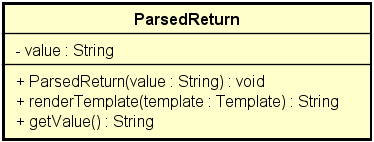
\includegraphics[scale=0.8,keepaspectratio]{img/server/ParsedReturn.png}}
\caption{\nogloxy{swedesigner::server::project::ParsedReturn}}
\end{figure}
\FloatBarrier
\begin{itemize}
\item \textbf{Descrizione}\\
questa classe descrive il comportamento di un blocco di ritorno di un metodo.
\item \textbf{Utilizzo}\\
dispone della possibilità di effettuare il render di un template in ingresso.
\item \textbf{Classi ereditate}:
\begin{itemize}
\item \hyperref[\nogloxy{swedesigner::server::project::ParsedInstruction}]{\nogloxy{\texttt{ParsedInstruction}}}
\end{itemize}
\item \textbf{Attributi}:
\begin{itemize}
\item \nogloxy{\texttt{- value: String}}
\\ Rappresenta il valore di un oggetto ParsedReturn, ossia ciò che viene ritornato da un metodo.
\end{itemize}
\item \textbf{Metodi}:
\begin{itemize}
\item \nogloxy{\texttt{+ getValue(): String}}
\\ Ritorna il valore del corrispondente oggetto ParsedReturn.
\item \nogloxy{\texttt{+ ParsedReturn(value: String)}}
\\ Costruisce un oggetto ParsedReturn.
\\ \textbf{Parametri}:
\begin{itemize}
\item \nogloxy{\texttt{value: String}}
\\ Rappresenta il valore che dovrà essere assegnato al campo dati value di un oggetto ParsedReturn.
\end{itemize}
\item \nogloxy{\texttt{+ renderTemplate(template: Template): String}}
\\ Traduce l'oggetto ParsedReturn in una stringa che rappresenta il codice di un particolare linguaggio di programmazione.
\\ \textbf{Parametri}:
\begin{itemize}
\item \nogloxy{\texttt{template: Template}}
\\ Riferimento alla particolare istanza di Template da utilizzare.
\end{itemize}
\end{itemize}
\end{itemize}

\subsubsubsection{\nogloxy{swedesigner::server::project::ParsedStatement}}
\label{\nogloxy{swedesigner::server::project::ParsedStatement}}
\begin{figure}[h]
\centering
\nogloxy{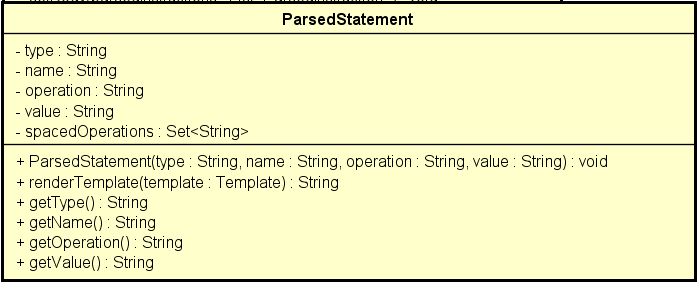
\includegraphics[scale=0.8,keepaspectratio]{img/server/ParsedStatement.png}}
\caption{\nogloxy{swedesigner::server::project::ParsedStatement}}
\end{figure}
\FloatBarrier
\begin{itemize}
\item \textbf{Descrizione}\\
questa classe descrive il comportamento di un blocco di assegnazione variabile o inizializzazione variabile.	
\item \textbf{Utilizzo}\\
dispone della possibilità di effettuare il render di un template in ingresso.
\item \textbf{Classi ereditate}:
\begin{itemize}
\item \hyperref[\nogloxy{swedesigner::server::project::ParsedInstruction}]{\nogloxy{\texttt{ParsedInstruction}}}
\end{itemize}
\item \textbf{Attributi}:
\begin{itemize}
\item \nogloxy{\texttt{- name: String}}
\\ Indica il nome dell'oggetto ParsedStatement.
\item \nogloxy{\texttt{- operation: String}}
\\ Indica l'operazione dell'oggetto ParsedStatement.
\item \nogloxy{\texttt{- spacedOperation: Set<String>}}
\\ Indica l'insieme di operatori legali utilizzabili nello statement.
\item \nogloxy{\texttt{- type: String}}
\\ Indica il tipo dell'oggetto ParsedStatement.
\item \nogloxy{\texttt{- value: String}}
\\ Indica il valore dell'oggetto ParsedStatement.
\end{itemize}
\item \textbf{Metodi}:
\begin{itemize}
\item \nogloxy{\texttt{+ getName(): String}}
\\ Ritorna il nome dell'oggetto ParsedStatement.
\item \nogloxy{\texttt{+ getOperation(): String}}
\\ Ritorna l'operatore dell'oggetto ParsedStatement.
\item \nogloxy{\texttt{+ getType(): String}}
\\ Ritorna il tipo dell'oggetto ParsedStatement.
\item \nogloxy{\texttt{+ getValue(): String}}
\\ Ritorna il valore dell'oggetto ParsedStatement.
\item \nogloxy{\texttt{+ ParsedStatment(type: String, name: String, operation: String, value: String)}}
\\ Costruisce un oggetto ParsedStatement.
\\ \textbf{Parametri}:
\begin{itemize}
\item \nogloxy{\texttt{type: String}}
\\ Rappresenta il tipo dell'oggetto ParsedStatement che si sta creando.
\item \nogloxy{\texttt{name: String}}
\\ Rappresenta il nome dell'oggetto ParsedStatement che si sta creando.
\item \nogloxy{\texttt{operation: String}}
\\ Rappresenta l'operazione dell'oggetto ParsedStatement che si sta creando.
\item \nogloxy{\texttt{value: String}}
\\ Indica il valore dell'oggetto ParsedStatement che si sta creando.
\end{itemize}
\item \nogloxy{\texttt{+ renderTemplate(template: Template): String}}
\\ Traduce l'oggetto ParsedStatement in una stringa che rappresenta il codice di un particolare linguaggio di programmazione.
\\ \textbf{Parametri}:
\begin{itemize}
\item \nogloxy{\texttt{template: Template}}
\\ Riferimento alla particolare istanza di Template da utilizzare.
\end{itemize}
\end{itemize}
\end{itemize}

\subsubsubsection{\nogloxy{swedesigner::server::project::ParsedType}}
\label{\nogloxy{swedesigner::server::project::ParsedType}}
\begin{figure}[h]
\centering
\nogloxy{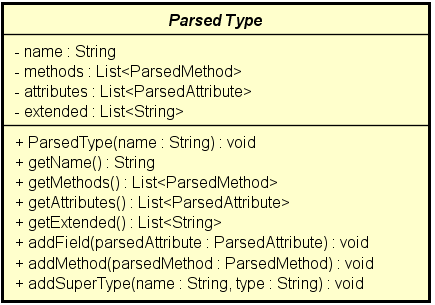
\includegraphics[scale=0.8,keepaspectratio]{img/server/ParsedType.png}}
\caption{\nogloxy{swedesigner::server::project::ParsedType}}
\end{figure}
\FloatBarrier
\begin{itemize}
\item \textbf{Descrizione}\\
questa classe astratta definisce un contratto comune tra le classi \texttt{ParsedInterface} e \texttt{ParsedClass}. 
\item \textbf{Utilizzo}\\
essa possiede un insieme di \texttt{ParsedMethod}. Nell'accezione di molti linguaggi, classi e interfacce rappresentano dei tipi. Questa classe deriva da \texttt{ParsedElement} al fine di poter usare polimorfismo sugli elementi creati dal \texttt{Parser}. 
I tipi sono creati dalla \texttt{ParsedFactory} e sono richiesti da \texttt{Parser}.
\item \textbf{Sottoclassi}:
\begin{itemize}
\item \hyperref[\nogloxy{swedesigner::server::project::ParsedClass}]{\nogloxy{\texttt{ParsedClass}}}
\item \hyperref[\nogloxy{swedesigner::server::project::ParsedInterface}]{\nogloxy{\texttt{ParsedInterface}}}
\end{itemize}
\item \textbf{Relazioni con altre classi}:
\begin{itemize}
\item \textit{IN} \hyperref[\nogloxy{swedesigner::server::project::ParsedProgram}]{\nogloxy{\texttt{ParsedProgram}}}\\
questa classe rappresenta l'entità che possiede al suo interno tutte le componenti di un progetto. Essa possiede più \texttt{ParsedType}.
\item \textit{OUT} \hyperref[\nogloxy{swedesigner::server::project::ParsedElement}]{\nogloxy{\texttt{ParsedElement}}}\\
questa classe descrive il contratto di un elemento generico \texttt{Parsed}. Si specifica il metodo \texttt{RenderTemplate} che impone la necessità di implementarlo ad ogni classe sottostante.
\item \textit{OUT} \hyperref[\nogloxy{swedesigner::server::project::ParsedMethod}]{\nogloxy{\texttt{ParsedMethod}}}\\
questa classe rappresenta un metodo come insieme di istruzioni \texttt{ParsedIstruction} e un insieme di \texttt{ParsedAttribute} come parametri del metodo.
\end{itemize}
\item \textbf{Attributi}:
\begin{itemize}
\item \nogloxy{\texttt{- attributes: List<ParsedAttribute>}}
\\ Rappresenta la lista dei campi dati di un particolare ParsedType.
\item \nogloxy{\texttt{- extended: List<String>}}
\\ Rappresenta l'insieme dei "supertipi" diretti estesi da un particolare ParsedType.
\item \nogloxy{\texttt{- methods: List<ParsedMethod>}}
\\ Rappresenta la lista dei metodi di un particolare ParsedType.
\item \nogloxy{\texttt{- name: String}}
\\ Rappresenta il nome di un particolare oggetto ParsedType.
\end{itemize}
\item \textbf{Metodi}:
\begin{itemize}
\item \nogloxy{\texttt{+ addField(parsedAttribute: ParsedAttribute): void}}
\\ Aggiunge all'oggetto ParsedType un campo dati rappresentato da un oggetto ParsedAttribute.
\\ \textbf{Parametri}:
\begin{itemize}
\item \nogloxy{\texttt{parsedAttribute: ParsedAttribute}}
\\ Rappresenta il campo dati da inserire in un particolare oggetto ParsedType.
\end{itemize}
\item \nogloxy{\texttt{+ addMethod(parsedMethod: ParsedMethod): void}}
\\ Aggiunge ad un oggetto ParsedType un metodo rappresentato da un oggetto ParsedMethod.
\\ \textbf{Parametri}:
\begin{itemize}
\item \nogloxy{\texttt{parsedMethod: ParsedMethod}}
\\ Rappresenta il metodo da inserire in un particolare ParsedType.
\end{itemize}
\item \nogloxy{\texttt{+ addSupertype(name: String, type: String): void}}
\\ Aggiunge il nome di uno dei "supertipi" diretti dell'oggetto ParsedType.
\\ \textbf{Parametri}:
\begin{itemize}
\item \nogloxy{\texttt{name: String}}
\\ Indica il nome del "supertipo" che deve essere implementato o esteso.
\item \nogloxy{\texttt{type: String}}
\\ Indica il tipo, classe o interfaccia, che deve essere rispettivamente esteso o implementato.
\end{itemize}
\item \nogloxy{\texttt{+ getAttributes(): List<ParsedAttribute>}}
\\ Ritorna la lista di campi dati di un particolare ParsedType.
\item \nogloxy{\texttt{+ getExtended(): List<String>}}
\\ Ritorna la lista dei supertipi diretti estesi da un particolare ParsedType.
\item \nogloxy{\texttt{+ getMethods(): List<ParsedMethod>}}
\\ Ritorna la lista dei metodi di un particolare ParsedType.
\item \nogloxy{\texttt{+ getName(): String}}
\\ Ritorna il nome di un particolare ParsedType.
\item \nogloxy{\texttt{+ ParsedType(name: String)}}
\\ Costruisce un oggetto ParsedType.
\\ \textbf{Parametri}:
\begin{itemize}
\item \nogloxy{\texttt{name: String}}
\\ Rappresenta il nome dell'oggetto ParsedType che si sta creando.
\end{itemize}
\end{itemize}
\end{itemize}

\subsubsubsection{\nogloxy{swedesigner::server::project::ParsedWhile}}
\label{\nogloxy{swedesigner::server::project::ParsedWhile}}
\begin{figure}[h]
\centering
\nogloxy{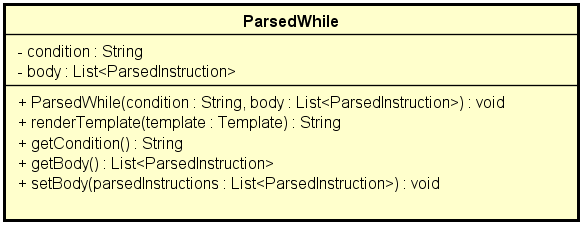
\includegraphics[scale=0.8,keepaspectratio]{img/server/ParsedWhile.png}}
\caption{\nogloxy{swedesigner::server::project::ParsedWhile}}
\end{figure}
\FloatBarrier
\begin{itemize}
\item \textbf{Descrizione}\\
questa classe descrive il comportamento di un blocco \texttt{while} e dispone della possibilità di effettuare il render di un template in ingresso.
\item \textbf{Utilizzo}\\
deriva da \texttt{ParsedInstruction}.
\item \textbf{Classi ereditate}:
\begin{itemize}
\item \hyperref[\nogloxy{swedesigner::server::project::ParsedInstruction}]{\nogloxy{\texttt{ParsedInstruction}}}
\end{itemize}
\item \textbf{Attributi}:
\begin{itemize}
\item \nogloxy{\texttt{- body: List<String>}}
\\ Indica l'insieme di istruzioni contenute nel corpo del corrispondente oggetto ParsedWhile.
\item \nogloxy{\texttt{- condition: String}}
\\ Indica la condizione del corrispondente oggetto ParsedWhile.
\end{itemize}
\item \textbf{Metodi}:
\begin{itemize}
\item \nogloxy{\texttt{+ getBody(): List<ParsedInstruction>}}
\\ Ritorna l'insieme di istruzioni contenute nel corpo di un oggetto ParsedWhile.
\item \nogloxy{\texttt{+ getCondition(): String}}
\\ Ritorna la condizione di un oggetto ParsedWhile.
\item \nogloxy{\texttt{+ ParsedWhile(condition: String, body: List<ParsedInstruction>)}}
\\ Costruisce un oggetto ParsedWhile.
\\ \textbf{Parametri}:
\begin{itemize}
\item \nogloxy{\texttt{condition: String}}
\\ Rappresenta la condizione dell'oggetto ParsedWhile che si sta creando.
\item \nogloxy{\texttt{body: List<ParsedInstruction>}}
\\ Rappresenta l'insieme di istruzioni contenute nel corpo dell'oggetto ParsedWhile che si sta creando.
\end{itemize}
\item \nogloxy{\texttt{+ renderTemplate(template: Template): String}}
\\ Traduce l'oggetto ParsedWhile in una stringa che rappresenta il codice di un particolare linguaggio di programmazione.
\\ \textbf{Parametri}:
\begin{itemize}
\item \nogloxy{\texttt{template: Template}}
\\ Riferimento alla particolare istanza di Template da utilizzare.
\end{itemize}
\item \nogloxy{\texttt{+ setBody(parsedInstructions: List<ParsedInstruction>): void}}
\\ Permette di assegnare un insieme di istruzioni al corpo di un oggetto ParsedWhile.
\\ \textbf{Parametri}:
\begin{itemize}
\item \nogloxy{\texttt{parsedInstructions: List<ParsedInstruction>}}
\\ Rappresenta l'insieme di istruzioni da inserire nel corpo del corrispondente oggetto ParsedWhile.
\end{itemize}
\end{itemize}
\end{itemize}
\subsection{\nogloxy{swedesigner::server::stereotype}}
\label{\nogloxy{swedesigner::server::stereotype}}
\subsubsection{Informazioni generali}
\begin{itemize}
\item \textbf{Descrizione}\\
Questo package offre le classi che descrivono ciò che caratterizza un particolare stereotipo. Queste classi derivano tutte da una classe base chiamata \texttt{Stereotype}. Le classi che definiscono come deve variare ogni stereotipo sono contraddistinte dal suffisso \texttt{Stereotype} (e.g. \texttt{BoardStereotype}). Si noti che tra queste classi non sono presenti dei legami, in quanto sono necessarie alla generazione del codice. La struttura degli stereotipi assegnabili ad ogni classe e le loro relazioni saranno definite successivamente nella \emph{Definizione di Prodotto}.
\item \textbf{Padre}: \hyperref[\nogloxy{swedesigner::server}]{\nogloxy{\texttt{server}}}
\end{itemize}

\subsection{\nogloxy{swedesigner::server::template}}
\label{\nogloxy{swedesigner::server::template}}
\subsubsection{Informazioni generali}
\begin{itemize}
\item \textbf{Descrizione}\\
Questo package contiene le classi necessarie a trasformare l'oggetto che rappresenta il programma in una stringa di testo che rappresenta il codice sorgente tramite un sistema a template, il quale definirà tramite dei file di testo la struttura di ogni componente del programma; per facilitare questo compito sarà usata la libreria \stringtemplate{}. Similarmente al package \texttt{Generator} si è prevista la possibilità di implementare un sistema di template per ogni linguaggio, implementando diversamente l'interfaccia della classe Template e definendo un nuovo package (e.g. \texttt{Java}).
\item \textbf{Padre}: \hyperref[\nogloxy{swedesigner::server}]{\nogloxy{\texttt{server}}}
\item \textbf{Package contenuti}:
\begin{itemize}
\item \hyperref[\nogloxy{swedesigner::server::template::java}]{\nogloxy{\texttt{java}}}\\
Questo package definisce le operazioni necessarie all'applicazione del template relativo al linguaggio Java. Simili package possono essere creati per permettere l'esportazione in diversi linguaggi target.
\end{itemize}
\end{itemize}
\subsubsection{Classi}
\subsubsubsection{\nogloxy{swedesigner::server::template::Template}}
\label{\nogloxy{swedesigner::server::template::Template}}
\begin{figure}[h]
\centering
\nogloxy{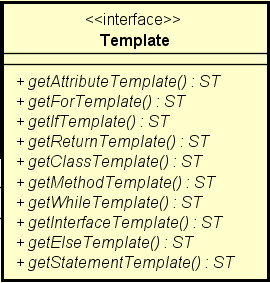
\includegraphics[scale=0.8,keepaspectratio]{img/server/Template.png}}
\caption{\nogloxy{swedesigner::server::template::Template}}
\end{figure}
\FloatBarrier
\begin{itemize}
\item \textbf{Descrizione}\\
questa interfaccia si occupa di fornire un oggetto template generico a chi lo richiede in modo da poter rendere estensibile il sistema aggiungendo un'implementazione concreta del template del linguaggio target desiderato.
\item \textbf{Utilizzo}\\
\texttt{RequestHandlerController} ha una dipendenza verso Template in quanto chiederà a \texttt{TemplateAssembler} una implementazione concreta di un \texttt{Template} in base al linguaggio target. Il pattern realizzato con questa classe è una \emph{dependency injection}.
\item \textbf{Relazioni con altre classi}:
\begin{itemize}
\item \textit{IN} \hyperref[\nogloxy{swedesigner::server::generator::Generator}]{\nogloxy{\texttt{Generator}}}\\
questa interfaccia si occupa di fornire un oggetto \texttt{Generator} generico a chi lo richiede in modo da poter rendere entensibile il sistema aggiungendo un'implementazione concreta del generator del linguaggio target desiderato.
\item \textit{IN} \hyperref[\nogloxy{swedesigner::server::template::java::JavaTemplate}]{\nogloxy{\texttt{JavaTemplate}}}\\
questa classe è una implementazione di \texttt{Template} che permette di fornire un template di una classe, metodo o costrutto Java.
\end{itemize}
\item \textbf{Metodi}:
\begin{itemize}
\item \nogloxy{\texttt{+ getAttributeTemplate(): ST}}
\\ Ritorna il template per tradurre un oggetto ParsedAttribute nel codice di un particolare linguaggio.
\item \nogloxy{\texttt{+ getClassTemplate(): ST}}
\\ Ritorna il template per tradurre un oggetto ParsedClass nel codice di un particolare linguaggio.
\item \nogloxy{\texttt{+ getElseTemplate(): ST}}
\\ Ritorna il template per tradurre un oggetto ParsedElse nel codice di un particolare linguaggio.
\item \nogloxy{\texttt{+ getForTemplate(): ST}}
\\ Ritorna il template per tradurre un oggetto ParsedFor nel codice di un particolare linguaggio.
\item \nogloxy{\texttt{+ getIfTemplate(): ST}}
\\ Ritorna il template per tradurre un oggetto ParsedIf nel codice di un particolare linguaggio.
\item \nogloxy{\texttt{+ getInterfaceTemplate(): ST}}
\\ Ritorna il template per tradurre un oggetto ParsedInterface nel codice di un particolare linguaggio.
\item \nogloxy{\texttt{+ getMethodTemplate(): ST}}
\\ Ritorna il template per tradurre un oggetto ParsedMethod nel codice di un particolare linguaggio.
\item \nogloxy{\texttt{+ getReturnTemplate(): ST}}
\\ Ritorna il template per tradurre un oggetto ParsedReturn nel codice di un particolare linguaggio.
\item \nogloxy{\texttt{+ getStatementTemplate(): ST}}
\\ Ritorna il template per tradurre un oggetto ParsedStatement nel codice di un particolare linguaggio.
\item \nogloxy{\texttt{+ getWhileTemplate(): ST}}
\\ Ritorna il template per tradurre un oggetto ParsedWhile nel codice di un particolare linguaggio.
\end{itemize}
\end{itemize}
\subsection{\nogloxy{swedesigner::server::template::java}}
\label{\nogloxy{swedesigner::server::template::java}}
\subsubsection{Informazioni generali}
\begin{itemize}
\item \textbf{Descrizione}\\
Questo package definisce le operazioni necessarie all'applicazione del template relativo al linguaggio Java. Simili package possono essere creati per permettere l'esportazione in diversi linguaggi target.
\item \textbf{Padre}: \hyperref[\nogloxy{swedesigner::server::template}]{\nogloxy{\texttt{template}}}
\end{itemize}
\subsubsection{Classi}
\subsubsubsection{\nogloxy{swedesigner::server::template::java::JavaTemplate}}
\label{\nogloxy{swedesigner::server::template::java::JavaTemplate}}
\begin{figure}[h]
\centering
\nogloxy{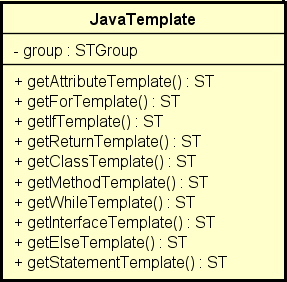
\includegraphics[scale=0.8,keepaspectratio]{img/server/JavaTemplate.png}}
\caption{\nogloxy{swedesigner::server::template::java::JavaTemplate}}
\end{figure}
\FloatBarrier
\begin{itemize}
\item \textbf{Descrizione}\\
questa classe è una implementazione di \texttt{Template} che permette di fornire un template di una classe, metodo o costrutto Java.
\item \textbf{Utilizzo}\\
viene utilizzata da \texttt{CompilerAssembler} che ritorna un' istanza di essa quando richiesto.
\item \textbf{Relazioni con altre classi}:
\begin{itemize}
\item \textit{OUT} \hyperref[\nogloxy{swedesigner::server::template::Template}]{\nogloxy{\texttt{Template}}}\\
questa interfaccia si occupa di fornire un oggetto template generico a chi lo richiede in modo da poter rendere estensibile il sistema aggiungendo un'implementazione concreta del template del linguaggio target desiderato.
\end{itemize}
\item \textbf{Attributi}:
\begin{itemize}
\item \nogloxy{\texttt{- group: STGroup}}
\\ Riferimento alla cartella da cui ricavare i file.st
\end{itemize}
\item \textbf{Metodi}:
\begin{itemize}
\item \nogloxy{\texttt{+  getMethodTemplate(): ST}}
\\ Ritorna il template per tradurre un oggetto ParsedMethod nel linguaggio Java.
\item \nogloxy{\texttt{+  getReturnTemplate(): ST}}
\\ Ritorna il template per tradurre un oggetto ParsedReturn nel linguaggio Java.
\item \nogloxy{\texttt{+ getAttributeTemplate(): ST}}
\\ Ritorna il template per tradurre un oggetto ParsedAttribute in linguaggio Java.
\item \nogloxy{\texttt{+ getClassTemplate(): ST}}
\\ Ritorna il template per tradurre un oggetto ParsedClass nel linguaggio Java.
\item \nogloxy{\texttt{+ getElseTemplate(): ST}}
\\ Ritorna il template per tradurre un oggetto ParsedElse nel linguaggio Java.
\item \nogloxy{\texttt{+ getForTemplate(): ST}}
\\ Ritorna il template per tradurre un oggetto ParsedFor nel linguaggio Java.
\item \nogloxy{\texttt{+ getIfTemplate(): ST}}
\\ Ritorna il template per tradurre un oggetto ParsedIf nel linguaggio Java.
\item \nogloxy{\texttt{+ getInterfaceTemplate(): ST}}
\\ Ritorna il template per tradurre un oggetto ParsedInterface nel linguaggio Java.
\item \nogloxy{\texttt{+ getStatementTemplate(): ST}}
\\ Ritorna il template per tradurre un oggetto ParsedStatement nel linguaggio Java.
\item \nogloxy{\texttt{+ getWhileTemplate(): ST}}
\\ Ritorna il template per tradurre un oggetto ParsedWhile nel linguaggio Java.
\end{itemize}
\end{itemize}
\subsection{\nogloxy{swedesigner::server::utility}}
\label{\nogloxy{swedesigner::server::utility}}
\subsubsection{Informazioni generali}
\begin{itemize}
\item \textbf{Descrizione}\\
Questo package contiene le componenti secondarie necessarie al server, indipendentemente dal linguaggio target dell'applicazione.
\item \textbf{Padre}: \hyperref[\nogloxy{swedesigner::server}]{\nogloxy{\texttt{server}}}
\end{itemize}
\subsubsection{Classi}
\subsubsubsection{\nogloxy{swedesigner::server::utility::Compressor}}
\label{\nogloxy{swedesigner::server::utility::Compressor}}
\begin{figure}[h]
\centering
\nogloxy{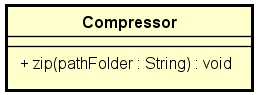
\includegraphics[scale=0.8,keepaspectratio]{img/server/Compressor.png}}
\caption{\nogloxy{swedesigner::server::utility::Compressor}}
\end{figure}
\FloatBarrier
\begin{itemize}
\item \textbf{Descrizione}\\
questa classe si occupa di creare e salvare su disco un archivio compresso contenente il progetto JSON, il codice sorgente e l'eseguibile generato che verrà poi messo a disposizione dell'utente che potrà scaricarlo.
\item \textbf{Utilizzo}\\
viene utilizzata da \texttt{RequestHandlerController} per creare l'archivio compresso dei file
\item \textbf{Relazioni con altre classi}:
\begin{itemize}
\item \textit{IN} \hyperref[\nogloxy{swedesigner::server::controller::RequestHandlerController}]{\nogloxy{\texttt{RequestHandlerController}}}\\
questa classe si occupa di ricevere le richieste REST provenienti dal client.
\end{itemize}
\item \textbf{Metodi}:
\begin{itemize}
\item \nogloxy{\texttt{+ zip(dirPath: String): void}}
\\ Crea una cartella zip contenente i file sorgenti e compilati del programma e la relativa stringa in formato .json.
\\ \textbf{Parametri}:
\begin{itemize}
\item \nogloxy{\texttt{dirPath: String}}
\\ Rappresenta la posizione della cartella, relativa ad una particolare richiesta, il cui contenuto verrà compresso in un file .zip.
\end{itemize}
\end{itemize}
\end{itemize}
